% Vorlage fuer Studien-, Bachelor- und Masterarbeiten am Lehrstuhl fuer Hochleistungsrechnen und IT Center, RWTH Aachen University
% Lehrstuhl fuer Betriebssysteme, RWTH Aachen University hat diese Vorlage erarbeitet
% basiert auf der Vorlage vom Lehrstuhl fuer Betriebssysteme
% basiert auf scrbook, Doku dazu im scrguide.pdf (texdoc scrguide  oder google)

\documentclass[12pt,             % Schriftgroesse
               a4paper,          % Papierformat
               %liststotoc,      % (alt) Tabellen- und Abbildungsverzeichnis im Inhaltsverz.
               listof=totoc,     % Tabellen- und Abbildungsverzeichnis im Inhaltsverz.
               %idxtotoc,        % (alt) Index im Inhaltsverz. auffuehren
               index=totoc,      % Index im Inhaltsverz. auffuehren
               %bibtotoc,        % (alt) Literaturverzeichnis im Inhaltsverz. auffuehren
               bibliography=totoc,% Literaturverzeichnis im Inhaltsverz. auffuehren
               %oneside,         % auskommentieren, wenn beidseitig gedruckt wird
                                 % default ist 'twoside'
               BCOR1cm,          % zusaetzlicher Bindungsrand
               %english,ngerman   % TODO : Englisch als weitere Sprache, Deutsch als Hauptsprache
               ngerman,english  % TODO : alternativ Deutsch als weitere und Englisch als Hauptsprache
               ]{scrbook}

%%%%%%%%%%%%%%%%%%%%%%%%%%%%%%%%%%%%%%%%%%%%%%%%%%%%%
% Pakete einbinden (Reihenfolge ist z.T. wichtig!)
%%%%%%%%%%%%%%%%%%%%%%%%%%%%%%%%%%%%%%%%%%%%%%%%%%%%%
\usepackage[latin1]{inputenc}   % Eingabezeichenkodierung, alternativ "ansinew"
                                %  (Windows only) oder "utf8" fuer Unicode
\usepackage{cmap}               % Fuer schoene Ligaturen in PDFs
\usepackage[T1]{fontenc}        % u.a. Umlaute als ein Zeichen in der PDF-Datei
\usepackage{lmodern}            % Linux Modern Schriften auswaehlen
\usepackage{graphicx}           % Um Bilder einzubinden (mit \includegraphics)
\usepackage{tikz}               % Um Latex Grafiken zu erstellen
\usepackage{makeidx}            % Falls ein Index erstellt werden soll, muessen
\makeindex                      %  die beiden Zeilen aktiviert werden.
                                %  zusaetzlich noch \printindex unten
\usepackage{units}              % Einheiten setzen mit z.B. \unit[10]{MB} und \unitfrac[100]{Mbit}{s}
%\usepackage{siunitx}           % Wesentlich umfangreicheres Einheiten Paket als Ersatz fuer "units"
\usetikzlibrary{arrows,shapes}  % Fuer Latex Grafiken
\usetikzlibrary{calc}


\usepackage{subfigure}
\usepackage{listings}
\usepackage{amsmath}
\usepackage{caption}
\DeclareCaptionFont{white}{\color{white}}
\DeclareCaptionFormat{listing}{\colorbox{gray}{\parbox{\textwidth}{#1#2#3}}}
\captionsetup[lstlisting]{format=listing,labelfont=white,textfont=white}

\usepackage[]{algorithm2e}
\usepackage{pgfplots}


% In dieser Datei koennen eigene Erweiterungen eingebracht werden
% HIER: Nur wenn noetig Datei my_includes.tex aendern
\input{my_includes.tex}         % Eigene Pakete und Definitionen laden

% letztes:     ----------------------------------------------------------------------------------------------------
\usepackage{hpcdasa}           % HPC-Vorlage fuer Bachelor-, Master- und Studienarbeiten 
                               %  mit Titelseite
% dieses sollte immer als letztes eingebunden werden, da es hyperref mitbringt 
% (welches wirklich das letzte ist)

%%%%%%%%%%%%%%%%%%%%%%%%%%%%%%%%%%%%%%%%%%%%%%%%%%%%%%%%%%%%%%%%%%%%%%%%%%%%%%%
% Hier beginnt das eigentliche Dokument
%%%%%%%%%%%%%%%%%%%%%%%%%%%%%%%%%%%%%%%%%%%%%%%%%%%%%%%%%%%%%%%%%%%%%%%%%%%%%%%
\begin{document}

%% Ein paar wichtige Details konfigurieren
%%----------------------------------------
% HIER: Details anpassen in my_config.tex
%
% my_config.tex
%
% Diese Datei dient dazu, die Vorlage anzupassen.
% TODO : alle Einstellungen anpassen.
%

% Ein paar Variablen f�r die Titelseite
\author{Till Schumann}                             % Name des Autors
\matnr{293576}                                       % Matrikel-Nummer
\reporttype{Masterthesis}                          % Studienarbeit/Diplomarbeit/Bachelorarbeit/Masterarbeit
\titleDe{Simulation eines M�usegehirns, auf Basis von Messdaten des Allen Institute for Brain Science, auf dem Gro�rechner Blue Brain 4}         % Deutscher Titel
\titleEn{Simulating the mouse brain model constructed from Allen Institute for Brain Science data on the Blue Brain 4}       % Englischer Titel
% bitte beide Titel eintragen.

%\addsupervisor{Prof.\,Dr.\,rer.\,nat. Matthias~S.~M\"{u}ller}       % Betreuer
%\addsupervisor{Prof. Dr. Matthias~S.~M\"{u}eller}      % weitere Betreuer (bei Bedarf)

% Falls es einen Zweitgutachter gibt
%\addsecondreferee{Univ.-Prof.\,Dr.\,rer.\,nat. Unbekannt} % Zweitgutachter

% Falls mehrere Institute die Arbeit betreuen
\addinstitute{hpc}{Lehrstuhl f\"{u}r Hochleistungsrechnen, RWTH Aachen University\\
IT Center, RWTH Aachen University}{(')}
\addinstitute{lfbs}{Computational and Systems Neuroscience (INM-6), Forschungszentrum J�lich GmbH}{(*)}
\addinstitute{lfbs}{Blue Brain Project, Ecole Polytechnique Federale de Lausanne}{(*)}
\addsupervisor[hpc]{Prof.\,Dr.\,rer.\,nat. Torsten Wolfgang Kuhlen}
%\addsupervisor[hpc]{Manni Mustermann}                               % Erstgutachter
\addsecondreferee[lfbs]{Prof.\,Dr. Markus Diesmann}               % Zweitgutachter
\addadviser[hpc]{PhD. Hristo Iliev}                               % Betreuer/ Assistent
%\addsecondadviser[hpc]{Dr. Fabien Delalondre}                               % Betreuer/ Assistent
               % TODO : bearbeite Einstellungen in my_config.tex

%%%%%%%%%%%%%%%%%%%%%%%%%%%%%%%%%%%%%%%%%%%%%%%%%%%%%
% Der Vorspann (andere Seitennummerierung)
%%%%%%%%%%%%%%%%%%%%%%%%%%%%%%%%%%%%%%%%%%%%%%%%%%%%%
\frontmatter

\maketitle                %Titelseite ausgeben
\cleardoublepage
\printversicherung        %Versicherung, dass Arbeit selbstaendig erstellt wurde


% TODO : die Abstracts sind optional.
% Falls Datei abstract.tex existiert, diese einbinden
\IfFileExists{abstract.tex}
	{\cleardoublepage\phantomsection\pdfbookmark{\abstractname}{abstract} %% fuegt ersten Abstract in die Bookmarks ein
	 \begin{otherlanguage}{ngerman}
\begin{abstract}
  Hier werden auf einer halben bis ganzen Seite die Kernaussagen der Arbeit
  auf Deutsch zusammengefasst.
  \bigskip\par
  \textbf{Stichw"orter:} HPC, OpenMP
\end{abstract}
\end{otherlanguage}
\begin{otherlanguage}{english}
\begin{abstract}
  Hier werden auf einer halben bis ganzen Seite die Kernaussagen Arbeit
  auf Englisch zusammengefasst.
  \bigskip\par
  \textbf{Keywords:} HPC, OpenMP
\end{abstract}
\end{otherlanguage}

	}{}


\cleardoublepage
\phantomsection\pdfbookmark{\contentsname}{toc}
\tableofcontents          %Inhaltsverzeichnis

\listoffigures            %Abbildungsverzeichnis

\listoftables             %Tabellenverzeichnis

%%%%%%%%%%%%%%%%%%%%%%%%%%%%%%%%%%%%%%%%%%%%%%%%%%%%%
% Der Hauptteil ("normale" Seitennummerierung)
%%%%%%%%%%%%%%%%%%%%%%%%%%%%%%%%%%%%%%%%%%%%%%%%%%%%%
\mainmatter
% Hier werden die Kapitel eingebunden
% TODO : weitere Kapitel in my_chapters.tex eintragen
% Hier die Kapitel des Hauptteils einf�gen
% Einf�hrungskapitel
%

\chapter{Introduction}

In 2014, the Neurorobotics team of the Blue Brain Project (BBP), project of the Ecole Federale Polytechnique Federale de Lausanne (EPFL), successfully produced a point-neuron model
of a mouse brain from data provided by the Allen Institute for Brain Science (Provide reference of Allen Institute).
Using NEST software, the BBP Neurorobotics team was then able to simulate a
scaled-down model of the mouse brain on a laptop computer, paving the way towards
making a mouse brain interact with an environment. A full-scale implementation of
the mouse brain model is possible, but requires the of large scale resources with low latency requirements only modern supercomputers can today provide.
The current functionality of NEST supports  generating large neuronal networks
on a super computer based an random distributions but not yet from experimental data contained in brain atlases. 
We suggest as part of this thesis to first develop the means to fully model a mouse brain from experimental data using NEST software on available supercomputing architectures.
\newpage

\section{Brain Simulations}
\section{Anatomy of the brain}
 
 The human brain is the main part of the central nervous system
 which consists of the spinal cord, sensory organs
 and all of the nerves that connect these organs with the rest of the body.
 These organs are responsible for the control of the body and communication between its parts.
 The nervous system is the most complex system of our body with respect to functionality.
 It contains billions of nerve and glia cells. 
 The nerve cells are connected via synapses to a complex network.
 Electrical pulses from neuron to neuron transmit information through the network.
 Glia cells help to maintain the right concentration of chemical substances in the
 extracellular space around neurons and provide supporting structures for the
 growth of neurons and for their spatial arrangement.
  \subsection{Macroscopic structure}
  \label{sec:Macroscopicstructure}
  The anatomy of the brain as depicted in Figure \ref{Aufbau1}, shows that different parts vary in cell density and functionality.
 Figure \ref{Aufbau1} shows a cross-section of the human brain. The outer layer is called the gray matter, due to the color caused by the high density of nerve cells.
 The white matter, which is underneath the gray matter,
 consists most of connection fibers of the nerve cells.
 The thalamus is situated in the middle of the brain and functions as a relay station between the sensory system and the cortical systems for cognition and motor control.
  \begin{figure}[!htbp]
  \subfigure[A cross-section of the human brain shows different densities of nerve cells \cite{CN}.]{
  \includegraphics[scale=0.3]{pictures/Aufbau1.png}
  \label{Aufbau1}
  }
  \hfill
  \subfigure[A general map of the human brain assigns parts of the gray matter to fuctionalities \cite{CN}.]{
  \includegraphics[scale=0.3]{pictures/Aufbau2.png}
  \label{Aufbau2}
  }
  \hfill
  \subfigure[The vertical structure of the gray matter shows six layers \cite{CN}.]{
  \includegraphics[scale=0.3]{pictures/mikro_aufbau.png}
  \label{mikroaufbau}
  }
  \caption{The macroscopic structure of the human brain.}
  \end{figure}
  Because of the high density of nerve cells the gray matter is the main part of information processing of the brain.
  
  The number of nerve cells (neurons), the number of connections (synapses) and the structure differs from person to person.
  The connections of each neuron are dynamic and change over time.
  Some parts of the brain can still be assigned roughly to functionality as shown in Figure \ref{Aufbau2}.\\
  Having a look at the vertical structure of the cortex,
  the gray matter can be partitioned in six layers as shown in figure \ref{mikroaufbau}.
  The cells in each layer have similarities like cell type, connections to other layers and connections to the thalamus and other parts.
  %-forebrain(anterior part of the brain)
  %-neocortex(surface of the mammalian brain, gray)
 
 
  \newpage
  \subsection{Microscopic structure}
  The nerve cells are tiny structures which are connected to each other.
  For an understanding of the brain a deeper look at the nerve cells is necessary.
  There are different cell types in a brain. They vary in structure and size.
  Pyramidal, spiny stellate and smooth stellate cells occur most often.
  For each layer there are types which occur more frequent. 
  
  In Figure \ref{Corticalneurons} a typical neuron is depicted.
  It contains the soma (the cell body) dendrites and axons.
  Electrical pulses are transported from the dendrites to the soma.
  In case of a spike an electrical impulse is forwarded through the axon.
  These axons are connected via synapses to further dendrites.
  The electrical impulse is transmitted via a chemical reaction in the synapse to the dendrites of connected cells.
  \begin{figure}[!htbp]
    \centering
    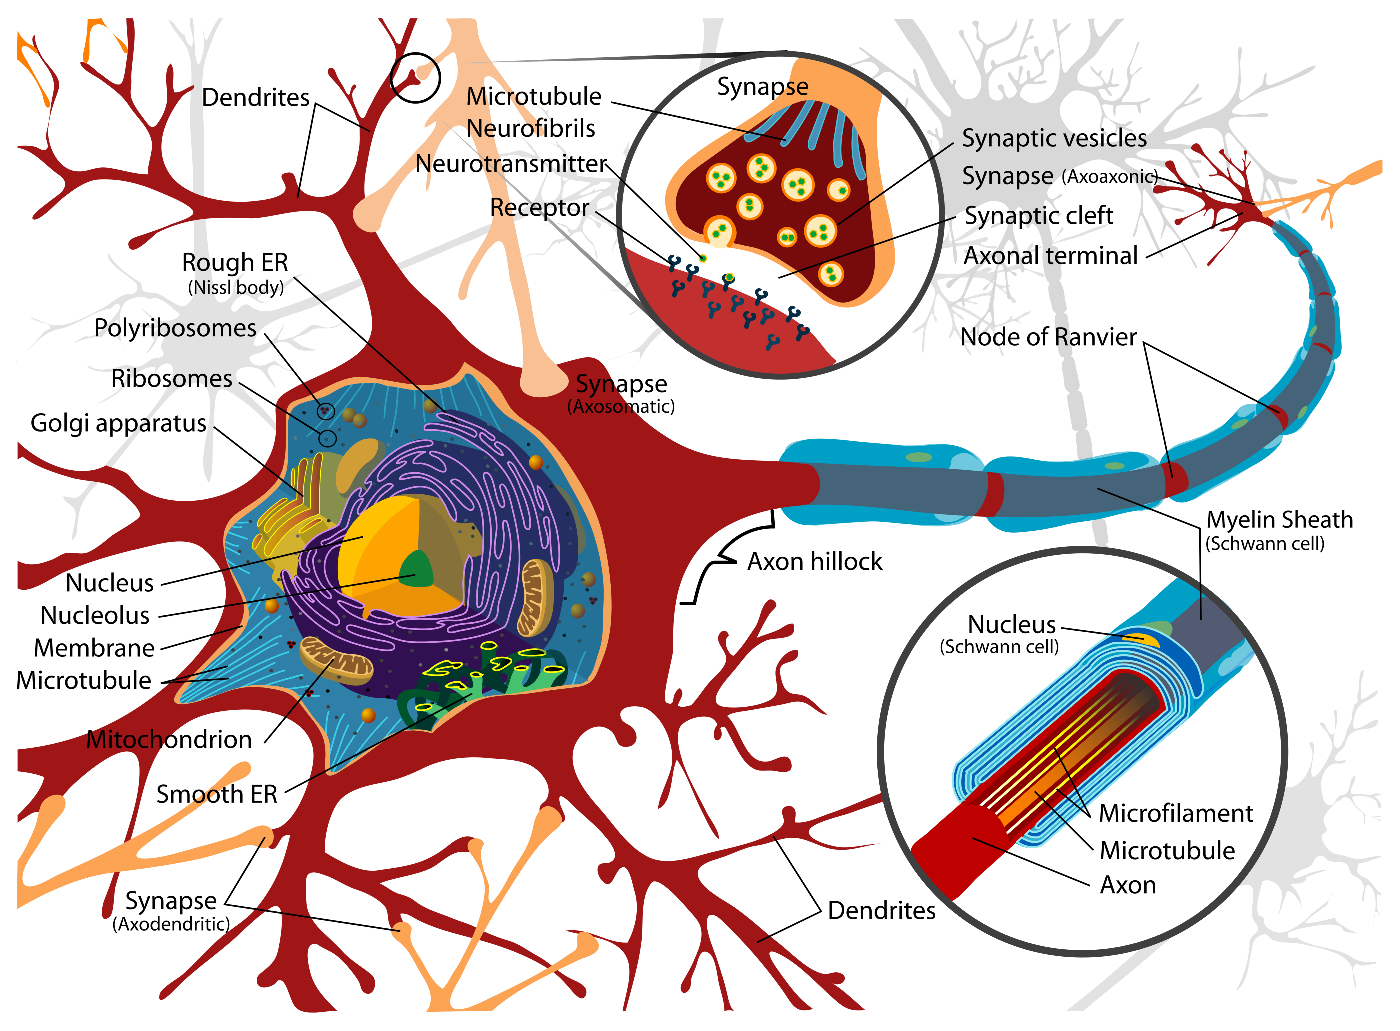
\includegraphics[scale=0.65]{pictures/Complete_neuron_cell_diagram_en.eps}
    \caption{Microscopic structure of a neuron. \cite{neuronpic}}
    \label{Corticalneurons}
  \end{figure}
  There are excitatory and inhibitory neurons.
  The excitatory neurons excite the following neurons, 
  in contrast the inhibitory neurons inhibit the following neurons.
  Via electrical currents the connected neurons influence the membrane potential of each neuron.
  The membrane potential can be measured.
  As an example the membrane potential is plotted over time in Figure \ref{membrane_potential}.
  Chemical processes inside the neuron generate a spike if the membrane potential reaches a specific electrical level called the threshold.  
  As shown in Figure \ref{membrane_potential} spikes are peaks in the membrane potential.  
  
  %-cortical neurons
  %-different cells: pyramidal, spiny stellate, smooth stellate
  %-cortical layers
  %-synapses
  
  %-10e12 neurons in the human brain
  \newpage
  \begin{figure}[!htbp]
  \subfigure[The plot shows the membrane potential of a neuron over the time.
  The peaks are called spikes.
  There are four spikes in the time span shown.
  The firing threshold of the cell is at about 58 mV \cite{CN}.]{
  \includegraphics[scale=0.36]{pictures/membrane_potential.png}
  \label{membrane_potential}
  }
  \hfill
  \subfigure[The dot plot shows spikes of each neuron over time. On the y-axis there are the neurons number.
  The histogram in the lower panel sums up all spikes for each time bin. \cite{CN}]{
  \includegraphics[scale=0.36]{pictures/spike_plot.png}
  \label{spikeplot}
  }
  \caption{The activity of a single neurons is displayed using its membrane potential. For multiple neurons the information is reduced to spike timings.}
  \end{figure}
  
  In order to analyze the membrane potential more objectively it is reduced to timings of the spikes.
  For multiple neuron the spike timings in a dot plot can be visualized as in Figure \ref{spikeplot}.
  One can get an overview of the activity in a whole neuronal network if the spike sums are
  plotted (summed up spikes for each time bin) in a so-called histogram.

	\begin{itemize}
      \item Short overview over simulators: NEST, NEURON, STEPS
      \item Possibilities/limits of simulations
   \end{itemize}
   
\section{Virtual mouse}
	\begin{itemize}
      \item Available data
      \item Why of interest
   	\end{itemize}   
\newpage
\section{Allen Brain Atlas}
   Allen Institute for Brain Science provides a high-resolution map of neural connections in the mouse brain.
   It contains several injection experiments. The provided datasets of the experiments 
   contain a 3D image of cell injection and a 3D image of its axonal projection labeled by viral
   tracers. So the images provide connection information between neurons all over the brain.
   The extracted connectivity information is used to build of long range connectivity inside
   the mouse brain model.
   
   \begin{figure}[ht!]
   	\begin{center}
        \subfigure[Injection sites - showing all available experiments]{%
            \label{fig:allInjections}
            \includegraphics[width=0.4\textwidth]{pictures/connectionBrowser_allinjections.png}
        }
        \hspace{1cm}
        \subfigure[Projection density of one experiment]{%
            \label{fig:oneProjection}
            \includegraphics[width=0.32\textwidth]{pictures/connectionBrowser_oneinjections.png}
       }
    	   \end{center}
    	\caption{%
        The pictures are inverted and copied from the Allen Brain Atlas.
     }%
   \label{fig:atlas}
   \end{figure}
   The figure \ref{fig:atlas} illustrate the given experiments and the projection image of an example experiment.
   They give an inside into the synaptic structure of the whole brain.
   
   \begin{itemize}
      \item description
\end{itemize}
   
   \newpage
\section{BBP recipe}

The BBP was able to reconstruct a microcircuit of somatosensory cortex of juvenile rat.
They presented a complementary algorithmic approach that reconstructs neuronal microcircuitry
across all layers using available sparse data and that leverages biological principles and
interdependencies between datasets to predict missing biological data.
The algorithm with the available data forms a recipe which is applied to the mouse
brain model to estimate the short range connectivity inside the mouse isocortex.
\begin{figure}[ht!]
\centering
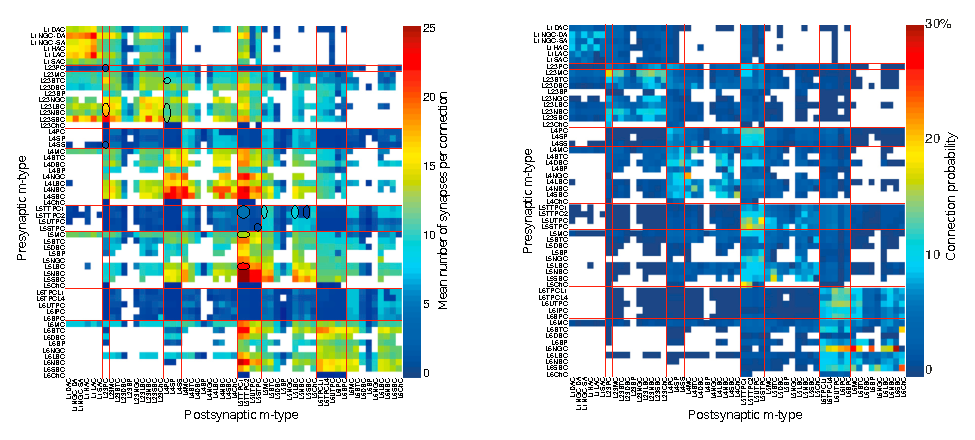
\includegraphics[scale=0.9]{pictures/BBPconnectionPropasMatrix.eps}
\caption{(Left) Synapses per connection. A matrix of the average synapses per connection for multi-synapse connections formed between the 55 m-types.
(Right) Connection probabilities. A matrix of average connection probabilities within 100 mm.}
\label{BBPconnectionPropasMatrix}
\end{figure}
The recipe is mainly based on probabilities of neuron types inside the somatosenory cortex.
The matrices in figure \ref{BBPconnectionPropasMatrix} shows the used matrices for \emph{m-type} for the neurons. 
To a given point neuron cloud with neuron type information the recipe returns synaptic
connections, which are used to extent the long range connectivity from the Allen Brain Atlas
by short range connectivity.

\section{NEST}
NEST is a simulator for spiking neural network models that focuses on the dynamics, size and structure of neural systems rather than on the exact morphology of individual neurons. The development of NEST is coordinated by the NEST Initiative. NEST is ideal for networks of spiking neurons of any size, for example:
Models of information processing e.g. in the visual or auditory cortex of mammals, models of network activity dynamics, e.g. laminar cortical networks or balanced random networks and models of learning and plasticity. A NEST simulation tries to follow the logic of an electrophysiological experiment that takes place inside a computer with the difference, that the neural system to be investigated must be defined by the experimenter. The definition is based on number of neurons with parameters and connections between these neurons. NEST supports the generation based on probabilistic values. The stochastic settings of a neuronal network can be used to create its artificial copy inside of NEST. To manipulate or observe the network dynamics, the experimenter can define so-called devices which represent the various instruments (for measuring and stimulation) found in an experiment. These devices write their data either to memory or to file. 

\section{Visualization}
To interpret the output of a neuronal simulation the spiking activity of the neurons is analyzed, mostly. 
Different types of methods allow to extract stochastic characteristics from spike trains.
Besides this visualization of the spike trains taking their location into account,
it can give an impression of the activity.

\begin{itemize}
      \item Visualization tools available
      \item BBP
      \item ViSNEST
\end{itemize}

% Ein Beispielkapitel
%

\chapter{Implementation}

The implementation which are done in this thesis enable to run the full mouse brain circuit.
Therefore a efficient data format is defined, the circuit generation scripts are adapted to
run on a bigger scale and the NEST simulator is extended to load the new data format.

\section{Data formats}

The data format for the neurons and the synapses follow two different concepts.
The neuron data format contains different datasets with the neuron parameters.
All datasets have to have the same length, which also defines the number of neurons.
The neuron parameters of neuron $i$ are stored in the i-th line of each data set.
Besides the data format contains attributes for storing meta data of the circuit.
\begin{figure}[ht!]
   	\begin{center}
        \subfigure[HDF5 file format for the neurons]{%
            \label{fig:allInjections}
            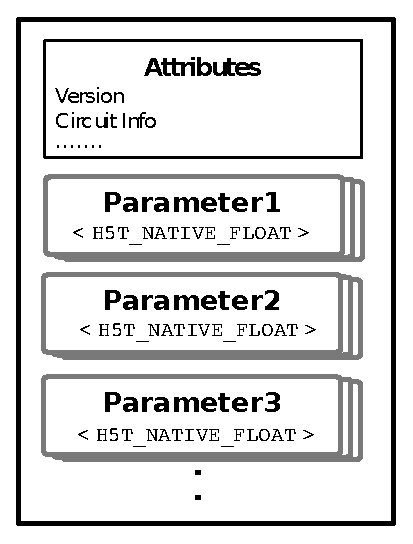
\includegraphics[scale=0.5]{pictures/hdf5_neuron_format.eps}
        }
        \hspace{1cm}
        \subfigure[HDF5 file format for the synapses]{%
            \label{fig:oneProjection}
            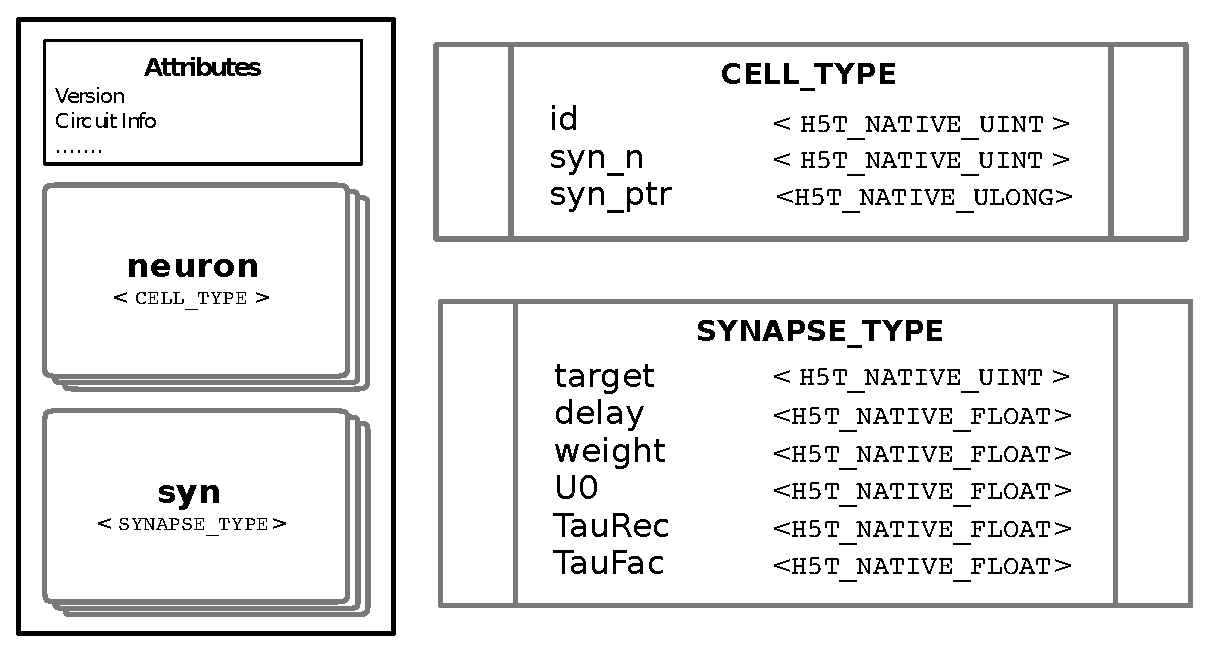
\includegraphics[scale=0.41]{pictures/hdf5_syn_format.eps}
       }
    	   \end{center}
    	\caption{%
        You can see the data format with their related datasets and data types. 
        How they are created by the circuit generation and loaded by the NEST import module.
     }%
   \label{fig:atlas}
   \end{figure}
The synapse data format contains only two datasets. In general the datasets contain for each synapse
a source neuron id, a target neuron id and a set of parameters. To reduce the amount of data.
The source neuron ids are grouped together in the \emph{neuron} dataset. This is feasible, because
the number of synapses is way bigger than the number of source neurons. The \emph{syn\_ptr} value 
defines the related starting index in the \emph{syn} dataset, respectively \emph{syn\_n} defines the
number of related following entries.
The \emph{syn} dataset contains the target neuron id and a set of parameters.
Both datasets use a compound data type to store different data types in the same dataset.

\newpage
\section{Circuit generation}
Rewriting the sequential python script to a hybrid C++ application require a parallel implementation of a parallelization strategy and the usage of 
a parallel random generator. For the parallelization strategy a Master-Slave approach is chosen to distribute the workload dynamically on the nodes.
Communication between the individual nodes is not necessary. Only the workload management is handled by the master node.
For the random generator Random123 is used, because it has good performance and it is easy to use \cite{salmon2011parallel}.
It ensures reproducible results without correlations in the generated values, which is essential.


\subsection{Long range connections}

The long range generation algorithm is adapted so it can be parallelized.
The problem with the sequential algorithm, that is iterates through all experiments
and generates all connections for all the voxels inside its injection regions, if 
all experiments before have not touched the voxels are have only higher total injection
value. This means it generates connections which might be overwritten and each iteration depends 
on all already completed iterations. To overcome this problem the best chosen injection is calculated before hand.
After that all voxels are distributed to the nodes and inside the iteration over all neurons
inside the given voxel, the sequential algorithm can be applied on each node.
Because the computation time needed by each voxel iteration varies a lot. Only the first third
of the voxels are distributed statically to the worker nodes.
All the other voxels are distributed dynamically by the master node.
The number of written entires can be calculated before hand. This allows to create
the HDF5 dataset before and assign a writing position to each voxel.
Thus all nodes can write independent to the file system.

\begin{itemize}
      \item parallelization strategy and implementation
      \item requirements 
\end{itemize}

\begin{figure}[ht!]
\centering
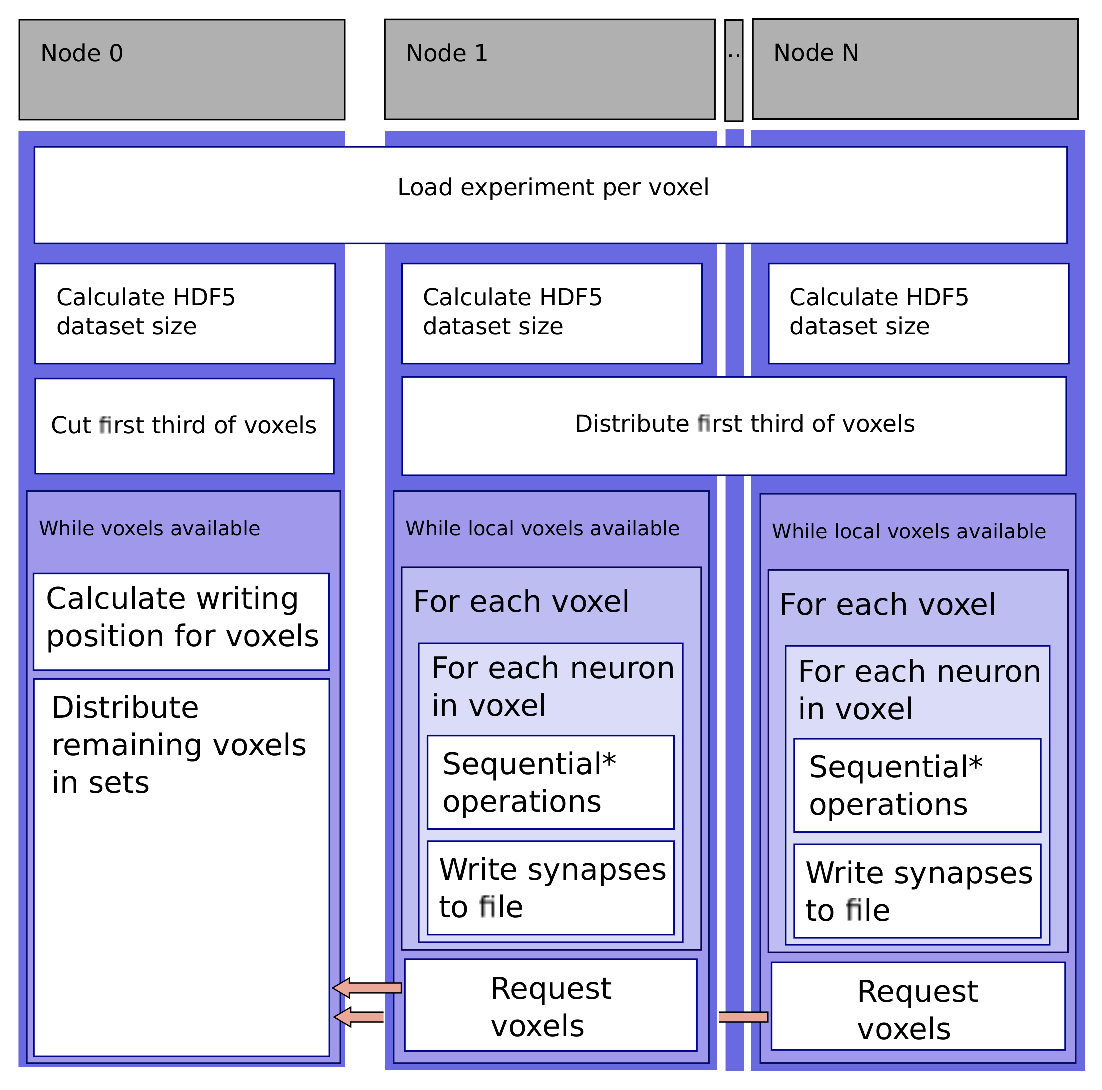
\includegraphics[scale=0.5]{pictures/longRange_parallelAlg.eps}
\caption{Task distribution between the nodes for the long range connections generation. It illustrates which tasks are distributed between which nodes.}
\end{figure}

\begin{figure}[ht!]
\centering
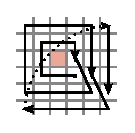
\includegraphics[scale=2.5]{pictures/longRange_Nearest_parallelAlg.eps}
\caption{Find nearest neighbor loop}
\label{longrange}
\end{figure}

The given algorithm was extended by a interpolation. There are voxels for which there is no injection of any experiment
available. To be able to generate connections for each neuron anyway. Voxels which are affected take the injection and projection from the nearest voxel with an injection. The strategy to find the nearest neighbor is an iteration around the neighborhood of each empty voxel. The Figure \ref{longrange} shows an illustration of the search algorithm
projected in a 2D plane. The first voxel along the search direction which is found is declared as ne nearest neighbor.


\begin{figure}[ht!]
\centering
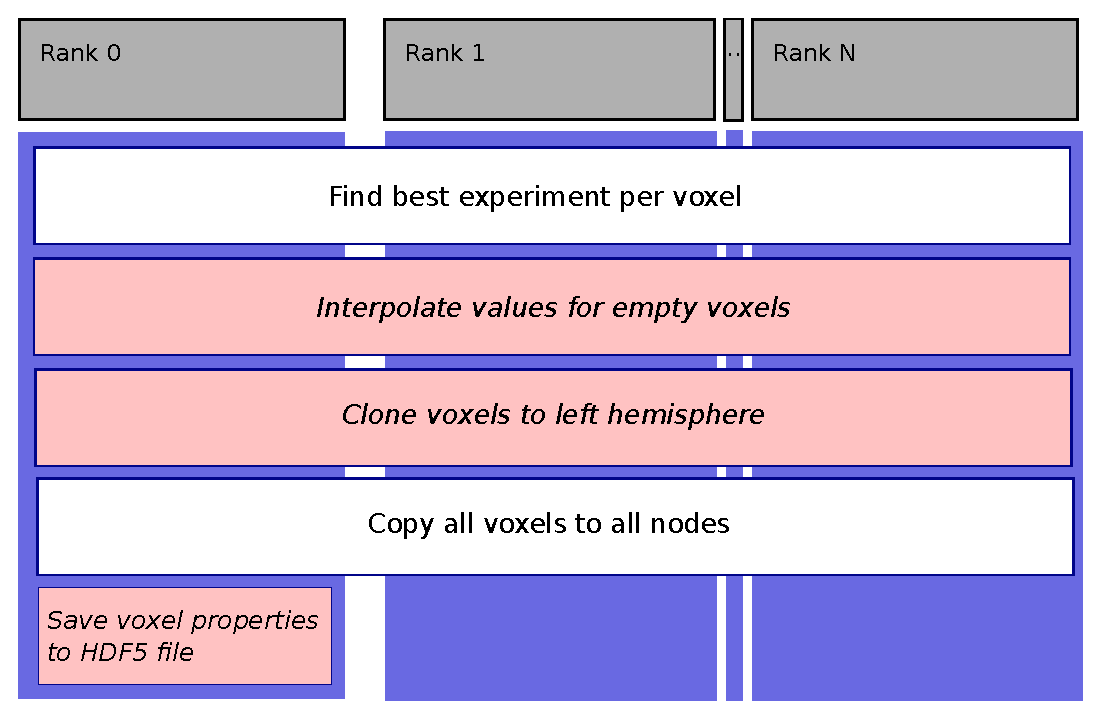
\includegraphics[scale=0.5]{pictures/longRange_BestExp_parallelAlg.eps}
\caption{Subtasks of the above listed \emph{Load experiment per voxel} task}
\end{figure}

\begin{figure}[ht!]
   	\begin{center}
        \subfigure[All nodes are equal and process the work based on a static distribution]{%
            \label{fig:shortColumn}
            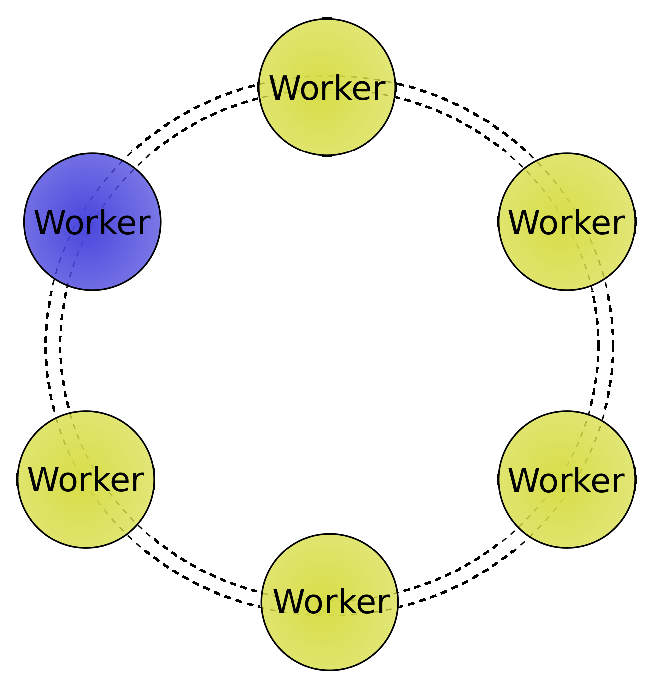
\includegraphics[scale=0.5]{pictures/All_Worker_Collective.eps}
        }
        \hspace{1cm}
        \subfigure[The 0 node is assigned as the master node and handles from this on the management of the work distribution.]{%
            \label{fig:shortColumnInCircuit}
            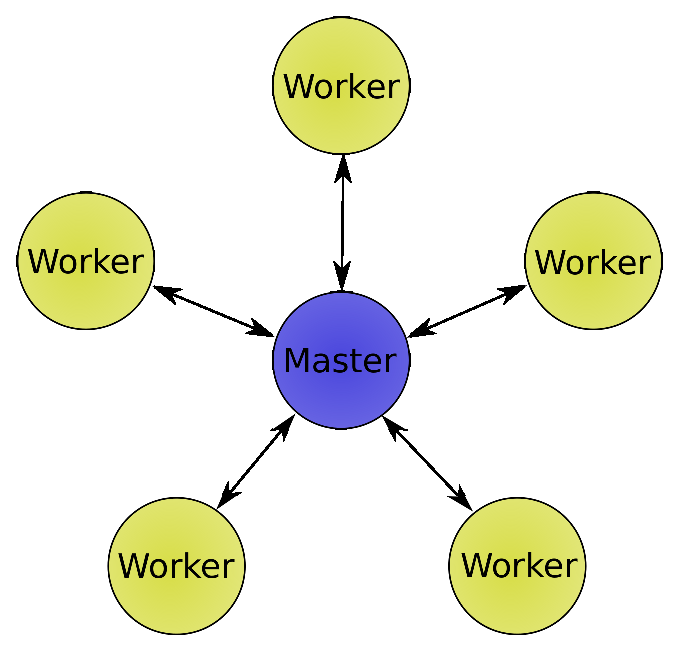
\includegraphics[scale=0.5]{pictures/MasterWorker.eps}
       }
    	   \end{center}
    	\caption{%
        The figure illustrates the work distribution and communication between the nodes.
     }%
   \label{fig:atlas}
   \end{figure}

\newpage
\subsection{Short range connections}

The algorithm presented in the analysis section can be parallelized straight forward.
Each iteration is independent. The challenging part is the distribution of the iterations and
the writing to disk. The number ob synapses which are created is not know. It is only available
at the end.

\begin{figure}[ht!]
\centering
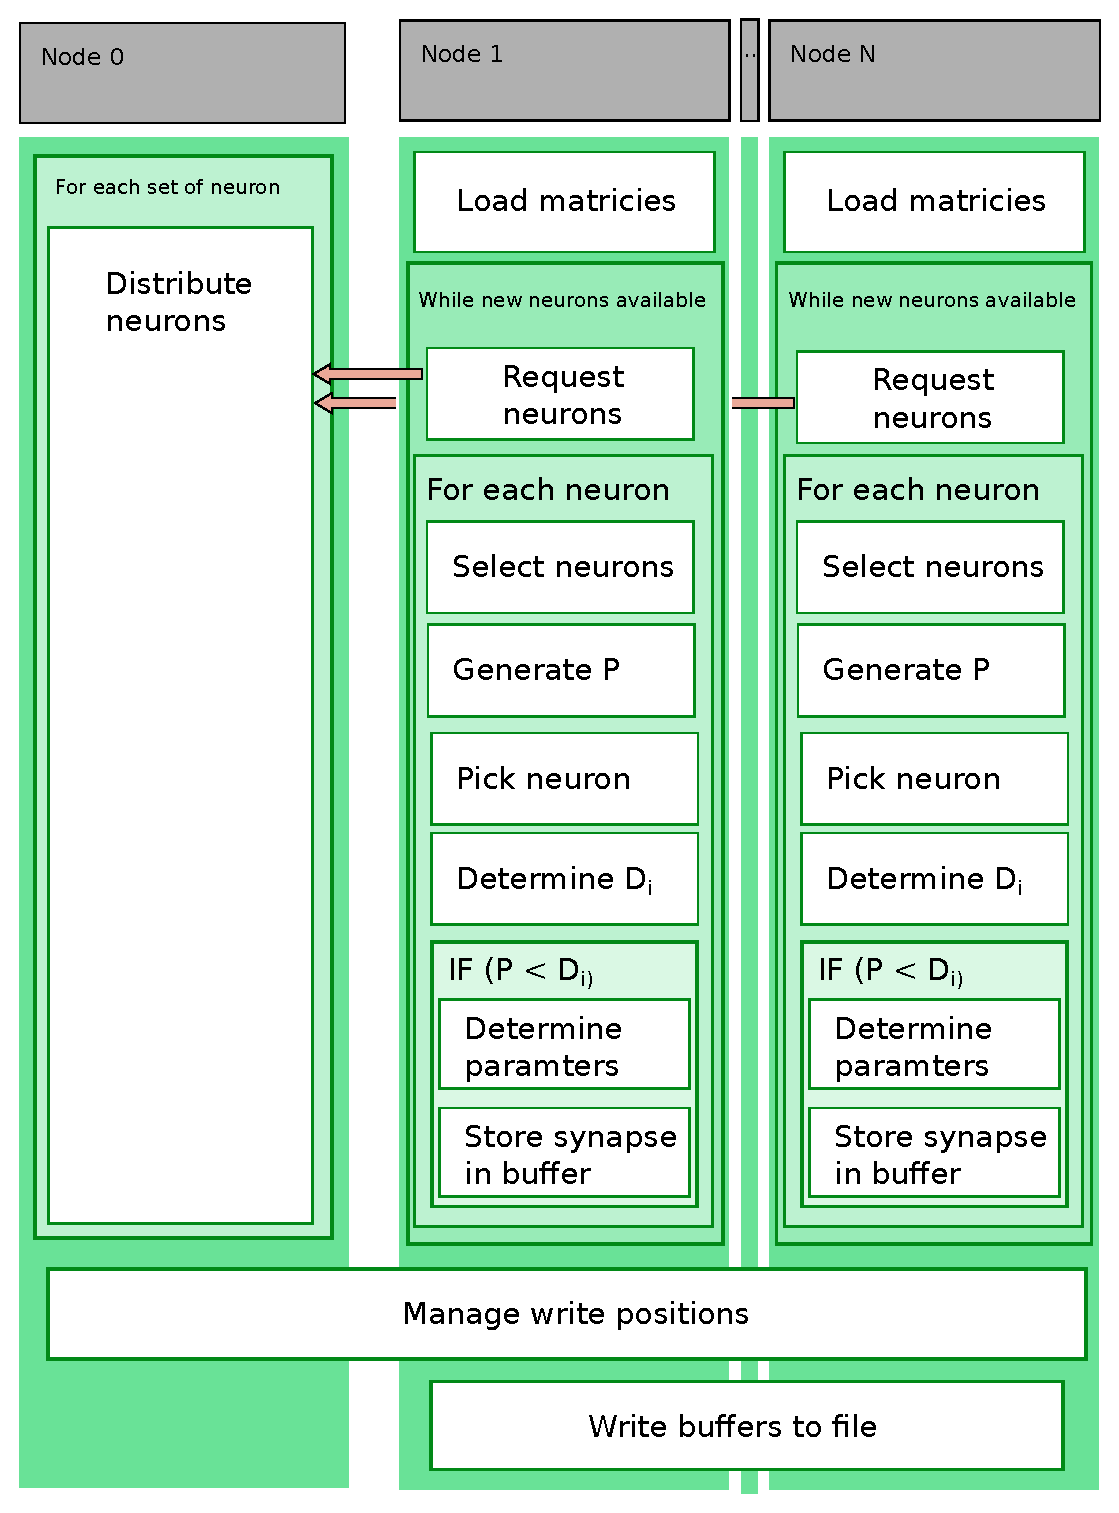
\includegraphics[scale=0.5]{pictures/shortRange_parallelAlg.eps}
\end{figure}

The short range algorithm is parallelized using a master-worker strategy to achieve a good load balancing.
The master node manages the distribution of the neurons, which can be seen as task units. For each neuron 
is synapses have to be created. The workers load in the first step all needed matrices from the file system.
Then each node request a set of neurons from the master node. Over this set it iterates and creates resulting
synapses. For \emph{Generate P} Random123 as a random number generator is used. Therefore a parallel usage of 
the given sequential algorithm is possible. Only the storage of the generated synapse list, has to be done 
after all iterations. So in each loop the synapse list is stored in a buffer.
If all neurons are distributed and processed all nodes, including the master node, calculate the position in 
the HDF5 dataset where each node is allowed to write. After that all workers write theirs synapse lists to
the HDF5 dataset.


\begin{figure}[ht!]
   	\begin{center}
        \subfigure[Master-worker strategy to get good balance properties]{%
            \label{fig:shortColumn}
            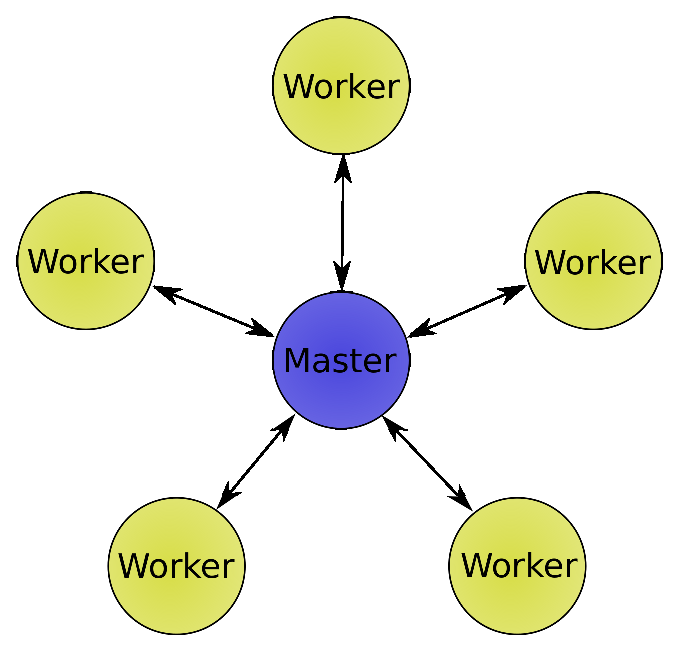
\includegraphics[scale=0.5]{pictures/MasterWorker.eps}
        }
        \hspace{1cm}
        \subfigure[Collective write operation to maximize used bandwidth]{%
            \label{fig:shortColumnInCircuit}
            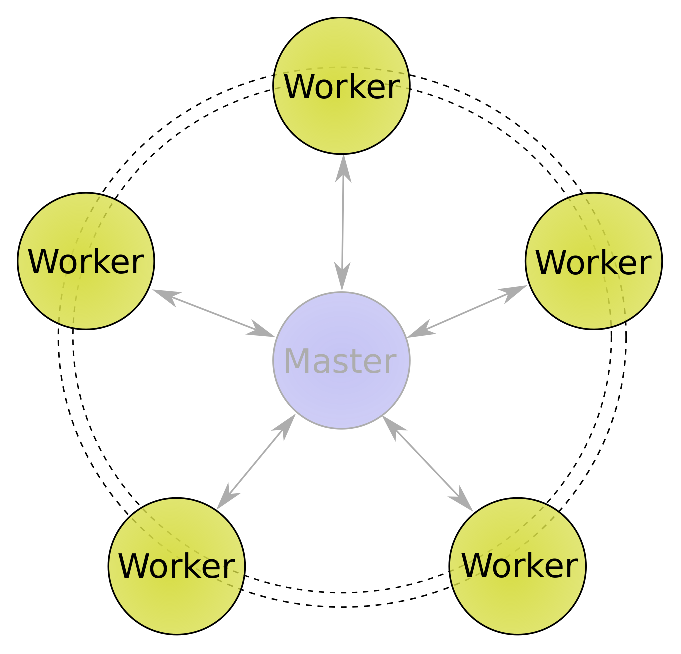
\includegraphics[scale=0.5]{pictures/Worker_Collective.eps}
       }
    	   \end{center}
    	\caption{%
        The figure illustrates the work distribution and communication between the nodes.
     }%
   \label{fig:atlas}
   \end{figure}
   
\begin{itemize}
      \item memory and computation requirements
\end{itemize}


\newpage
\section{Circuit validation}

In the context of this thesis the circuit is validated in terms of geometrical correct placement of
the synapses. So the position of the source and target can be visualized and be compared to a 
reference system. For the long and the short range connectivity the geometrical shape is know.
In particular the long range connectivity should connect neurons from the injected regions to neurons
in the projected region for each used experiment. Therefore a circuit for a single experiment is 
generated, the target and source neurons are visualized in a 3D coordinate system and the the injection
and projection is used as the reference system. If source neurons are inside the injection space and all
target neurons are in the projection space, the implementation works fine.
For the short range connectivity all post-synaptic neurons of synapses having the same pre-synaptic neuron should
lay inside a cylinder in layer 1 to 6. For the validation. 
 
\begin{itemize}
      \item Visual validation of synapses to identify neuron id miss interpretation
      \item Visual validation of spiking activity
      \item Statistical properties are not analyzed in this work 
\end{itemize}

\begin{figure}[ht!]
\centering
\includegraphics[width=0.4\textwidth]{pictures/paraview_ex.png}
\end{figure}

\section{NEST import modules}

The neuronal spiking network simulator NEST is developed in \emph{C++} and delivers
an user interface based on an own description language \emph{SLI} and  and a Python interface.
The new use case shall be integrated into the standard work flow of NEST.
Besides the functionality in \emph{C++} the interfaces have to be extended.
The difficulties of the network generation is based on a difference in 
the NEST internal data structure and the data delivered by the Allen Institute.
Connection information contains target and source neurons besides biochemical
information of the synapses. Because of the in vitro injection methods the
connection information maps the synapse from the source to the target neurons.
For multi process simulations NEST distributes all neurons based on a modulo function 
to the processes. Because of memory optimizations the synapses are only stored on the
post synaptic process. This means that the connection information is stored
on the process, where the target neuron is located. Therefore a transformation of the given data is
necessary. Preprocessing of the input data should be avoided as far as possible to capture
future use cases.
The resulting implementation shall load the connection information efficiently in parallel,
distribute the synapse information to the post synaptic node and store it in
the NEST data structure.
Further requirements of the implementation are an efficient use of the available resources as
memory and computation power. 


\subsubsection{Import neurons}
To import neurons into NEST using the internal C++ API NEST has to create the requested number of neurons and
assign their parameters afterwards. In an distributed environment the create function has to be called on all nodes. But assigning the parameters has only be done on the nodes, where the neurons are assigned to.
Thus only a set of the parameter datasets is needed on each node.
To group neurons together to subnets, subnets has to be created before the neurons are created.
This follows in the following algorithm.

\begin{algorithm}
 \KwData{HDF5 neuron dataset}
 \KwResult{Created neurons inside NEST data structure}
 Find unique values in subnet dataset; \\
 Create subnet for each unique entry; \\
 Create neurons based on length of HDF5 datasets with given neuron type inside specified subnets; \\
 Read parameter datasets collectively; \\
 Assign parameters to neurons;
\label{alg2}
\caption{}
\end{algorithm}

The distribution of the neurons to the nodes is known. NEST distributes the neurons based on the modulo of their ids. Neuron $i$ is placed on node $i mod number\_of\_nodes$. Each node has to load all needed parameter entries
from the datasets. Derived from the distribution function each node has to load each number\_of\_nodesths entry
starting from its node id.

\subsubsection{Import synapses}
Synapse import module reads the the synapse dataset block wise. Using hyperslabs each node selects a block from the
dataset and copy it to memory with all the specified parameters.
The source neuron list and the target neurons and their parameters from each block are used to create a list of all synapses.
For each entry the target node is determined.
The list is sorted by the target nodes.
Using \emph{MPI\_Alltoall} the list can be distributed directly to the corresponding nodes.
Afterwards each node contains its list of synapses and can use the \emph{NEST} connect function, to copy it to its internal data structure.
\begin{algorithm}
	\KwData{List of HDF5 files for each node, chunk size}
	\KwResult{Connected NEST network}
	\While{Chunk to read in HDF5 files}{
		Read block and store in memory \hspace{45px}(1)\;
 Create list of synapses (1,2) \hspace{36px}$\mathcal{O}(n)$\;
 Determine target node for each synapse \hspace{63px}(2,3) \hspace{36px}$\mathcal{O}(n)$\;
 Sort synapses by target nodes \hspace{66px}(2,3,*) \hspace{28px}$\mathcal{O}(n^2)$\;
 MPI\_Alltoallv using sorted list \hspace{76px}(2,3,4,5)\;
 Connect all synapses using NEST function \hspace{36px}(5) \hspace{45px}$\mathcal{O}(n)$\;
	}
\label{alg2}
\caption{Distribute connection information without transposing, $S_i$ source neuron $i$, $Tn_i$ target neuron $i$.
	set in brackets contains current needed variables}
\end{algorithm}

\begin{figure}[ht!]
\centering
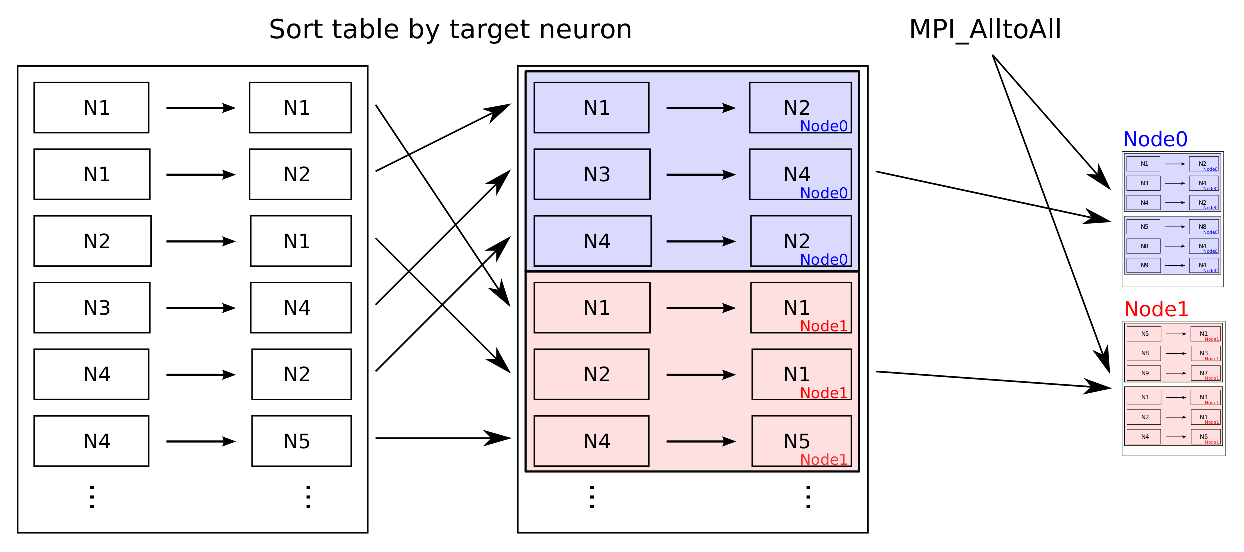
\includegraphics[scale=0.7]{pictures/sort_table_all_alltoall.eps}
\caption{Distribute synapses to the nodes.}
\end{figure}

\section{Memory consumption}
\begin{figure}[ht!]
\begin{tabular}{| l | l | l | l |}
    \hline
    (id) & data structures & memory consumption \\ \hline
    (1) & chunk in memory & $L_0 + h*(L_0 + L_S*w)$ \\ \hline
    (2) & connection table & $2*(L_0+L_S*w*s)$ \\ \hline
    (3) & target neuron node map & $L_0+L_S*w*s$ \\ \hline
    (4) & MPI send vectors & $L_0+L_S*2*w*s+2*(L_0+L_S*N)$ \\ \hline
    (5) & MPI recv vectors & $L_0+L_S*2*\frac{w*s}{\nu}+2*(L_0+L_S*N)$ \\ \hline
    \end{tabular}
\caption{$L_0$: constant memory overhead of list; $L_S$: memory consumption of entry type; $N$: number of nodes $w$: 1 dim of chunk; $h$: 2 dim of chunk; $DNC(w)$: replication of target neurons in chunk; $\nu$: distribution coefficient of data}
\end{figure}
The maximum memory consumption is:
\begin{equation}
  M = 9*L_0 + 4*L_S*N+L_S*w*s*(4+\frac{1}{\nu})
  \label{eq:maxmemoryconsumption}
\end{equation}
% Zusammenfassung und Ausblick
%

\chapter{Discussion}

\section{Circuit properties}


The generated full mouse brain circuit contains around 74 million neurons and 660 billion synapses.
From the neuron HDF5 file 12 parameters are used by the simulation.
It contains further parameters which are used for the connection generation and the visualization,
like coordinates. In total the neuron HDF5 file is of the size of around 9 GB.
The synapse HDF5 file only contains needed parameters for the simulation.
There are five synapse parameter per connection. This results in 15 TB of data
for the long range connectivity and 600 GB for the short range connectivity.
So the generated circuit contains around 15 TB and is spitted in three HDF5
files (neuron file, long range synapses file and short range synapses file).

The interpolation, which are applied to the circuit long range connection generation, introduces errors.
For illustration Figure \ref{interpolationdistance} shows the locality of missing voxels in one slice.
The quality of the interpolation can be estimated from the distance (color scale in Figure).
The distance corresponds to the distance from the nearest neighbour search algorithm.
It highlights problematic regions.
\begin{figure}[ht!]
\centering
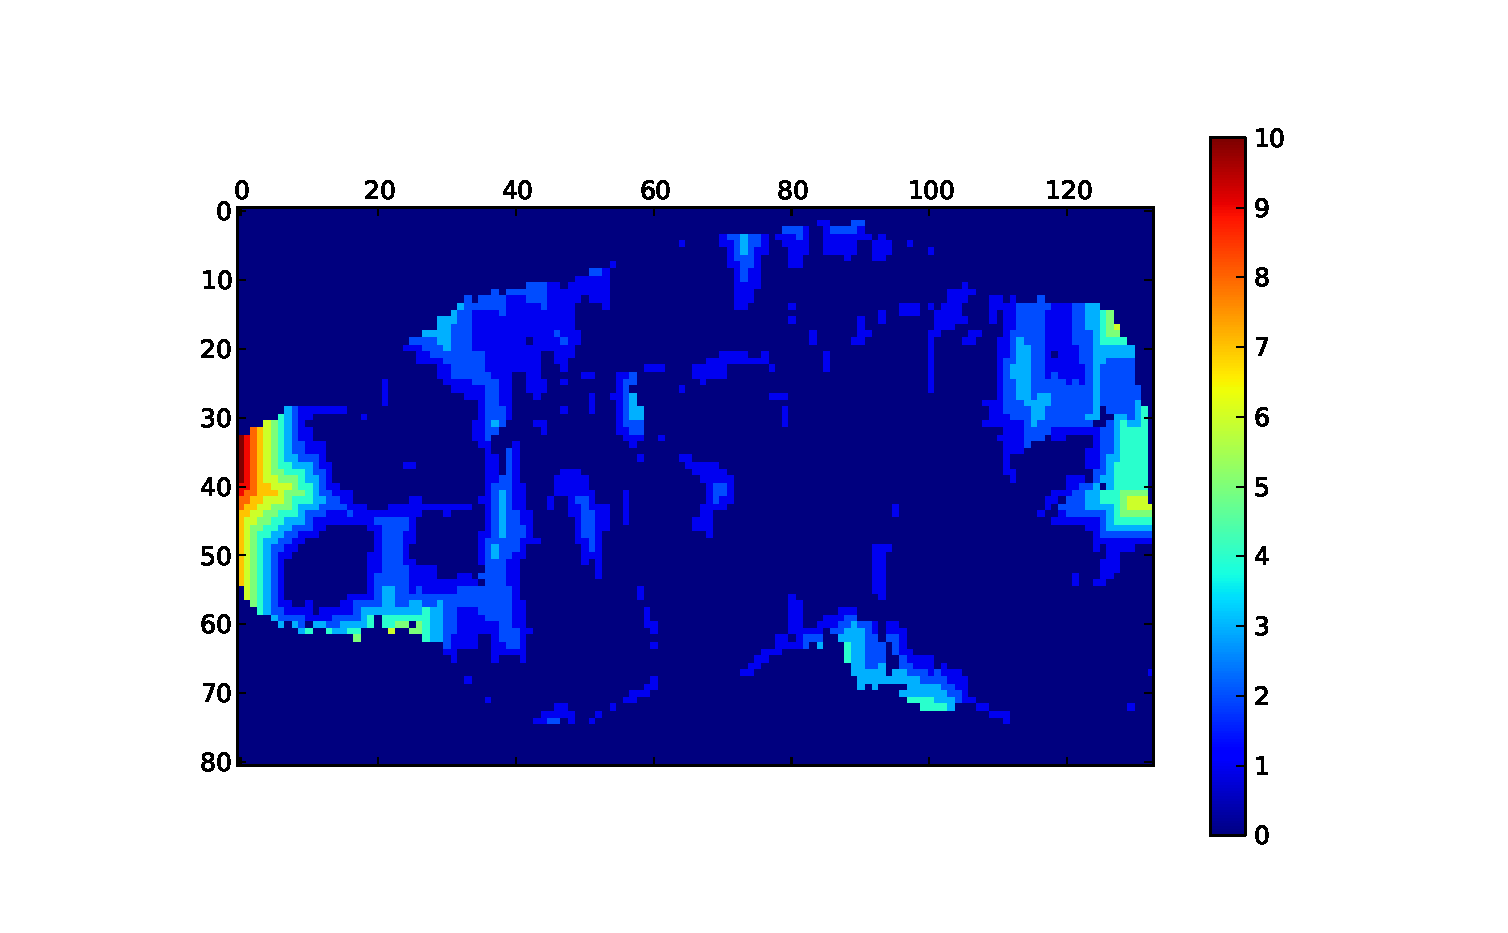
\includegraphics[scale=0.5]{pictures/distance_x_y_70.eps}
\caption{Plotted values from the nearest neighbor algorithm. You can see the distance to the next injected voxel.}
\label{interpolationdistance}
\end{figure}
It should be taken into account by analysing the circuit spiking activity
(the distance values are written to the voxel information file (\ref{file:voxelinfo})).
The interpolations allow to generate a full mouse brain model from incomplete experimental data.
A first simulation of a full circuit model is possible.
So the pipeline from Allen Brain and Blue Brain Project recipe data to a neuronal simulation with NEST can be tested.
If there are more experiments available they can be included into
the circuit generation easily.
It wont have an impact on the size of the resulting model.

\begin{table}[ht!]
\begin{centering}
    \begin{tabular}{ | l | l | r | r | r |}
    \hline
    Identifier & ratio & neurons & synapses & total size \\ \hline \hline
    threehundredths & $0.3\%$ & $~2.5*10^5$ & $~2.2*10^9$ & $~26$ GB \\ \hline
    quater & $25\%$ & $~1.9*10^7$ & $~1.6*10^{11}$ & $~4$ TB \\ \hline
    full & $100\%$ & $~7.5*10^7$ & $~7.2*10^{11}$ & $~16$ TB \\ \hline
    \end{tabular}
    \caption{The circuits \emph{3hundredths}, \emph{1quater} and \emph{full} were created for testing and debugging on different scales.
All circuits were generated with identical parameters, only the input neuron file varies.}
\end{centering}
    \end{table}


\label{table:circuits}

Three different circuits (see Table \ref{table:circuits}) are generated: The full mouse brain circuit,
a smaller circuit, which contains 25 percent of the full mouse brain circuit and
$\frac{1}{300}$ of the full circuit. The percentage is related to the number of neurons inside
the circuit. Based on the neurons the connections are generated. In principle the
number of connections should be of the same proportion.

\begin{figure}[ht!]
\centering
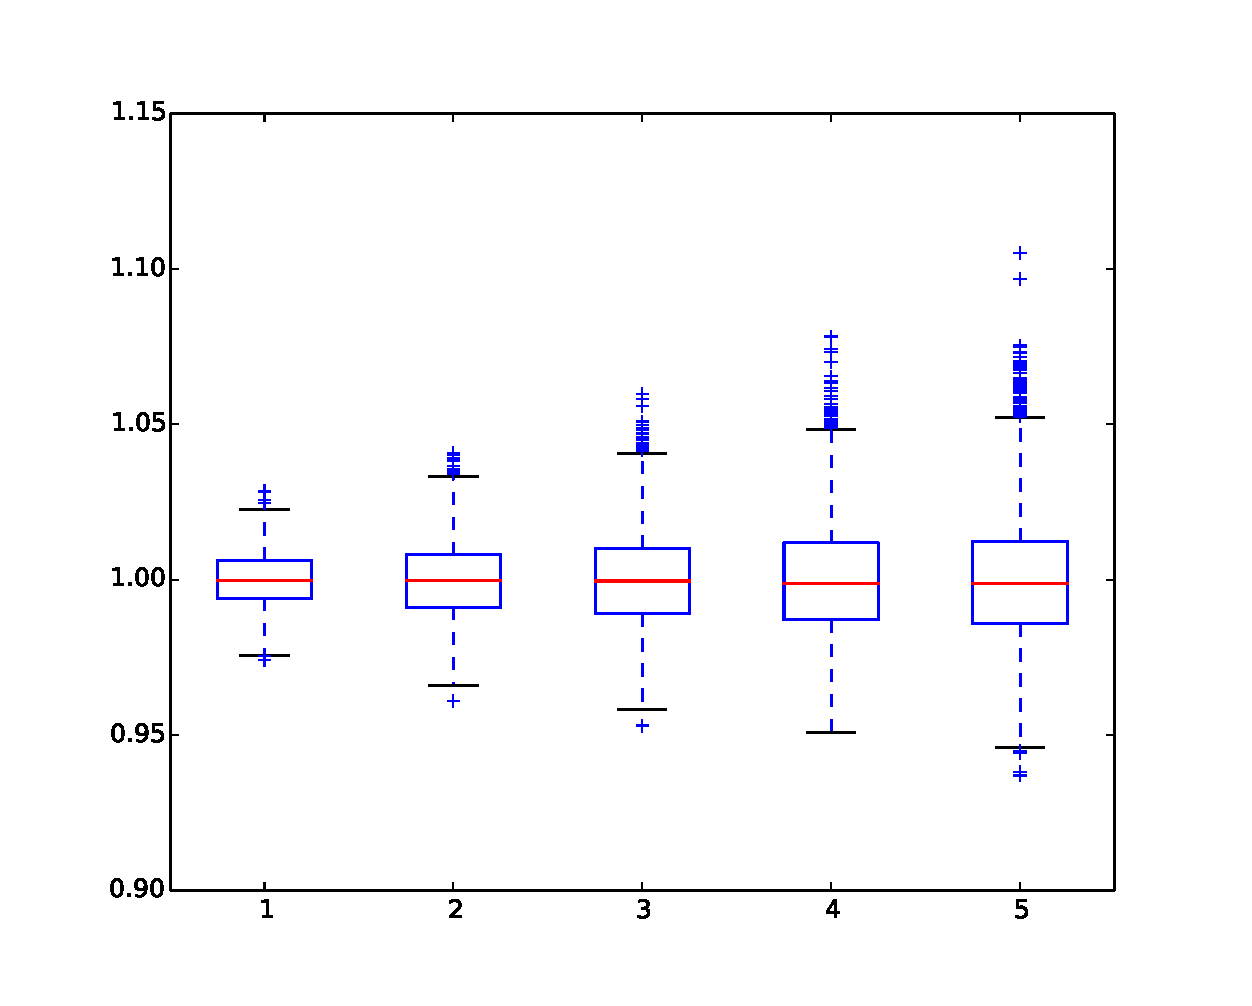
\includegraphics[scale=0.4]{pictures/full_circuit_rack_distribution.eps}
\caption{Estimated synapse imbalance of neuron distribution on processes.
It shows the distributions of relative sums (sum of number of synapses per process divided by mean of sums) of synapses per process (y-scale) on different scales (x-axis). Relative sums means absolute sums devided by the mean sum per process. }
\label{fullcircuitdist}
\end{figure}

The neurons are distributed equably on all processes based on equation \ref{eq:ProcessByNeuron}.
But the number of incoming synapses varies between the neurons.
Therefore a memory imbalance could occur between the processes.
To analyse the imbalance, an analysing script iterates over the \emph{syn} dataset and counts
the number of incoming synapses per neuron. Normalized results are plotted in box-plot diagrams 
in Figure \ref{fullcircuitdist}.
It shows an increasing imbalance of synapses per process with increasing number of processes.



\section{Data format usability}
The HDF5 data format for neuron parameters is used as given from the Neurorobotics team.
Because of its small size (9 GB) in comparison to the synapse dataset (15 TB) the performance improvement by changing
to a transposed data format can be neglected. Thus the usability of having different datasets and being able
to add new datasets can be kept. It also implies that the generation script does not have to be converted or no 
conversion scripts are needed.


\section{Long range connections generation}
The sequential algorithm is optimized and parallelized.
Moving the best injection per voxel search outside the main iteration
avoids unnecessary calculations and reduces the complexity of the main iteration.
In the sequential algorithm parts of the connections are regenerated in each iteration.
This is avoided by looking for the best injection per voxel beforehand.


Optimization of the linear acceptance rejection function (see \ref{par:linearacceptancerejection})
reduces the complexity of the picking from number of neurons in projection to number of voxels in projection.
For the full circuit this corresponds to a reduction of the order of 2.
Using all core inside the function gives a further speed up.
Each thread has to pick $~\frac{10,000}{N_{threads}}$ voxels instead of
$10,000$.



\section{Short range connections generation}
The sequential algorithm could be ported directly to a parallel implementation without changing it.
Using a Master-Slave approach also reduced the complexity of the distribution of independent iterations.
The only issue is the writing of the file, because the number of created synapses is not know in the beginning.
Using a buffer or temporary files is necessary to return a non chunk based HDF5 file.
Because of the given resources (IBM Blue Gene Q) and the high parallel efficiency (see later section)
wirting all synapses to memory is feasible (already for a small number of nodes the created connections fit in memory).

\section{Import circuit}
Four parts of the synapse loading algorithm are instrumented to get wall clock timings.
\emph{Read}, \emph{Sort}, \emph{Alltoall} and \emph{Connect} are considered to be the mots time
consuming parts of the algorithm. The parts relate to figure \ref{Algparts}.
\emph{Def. Node} is negligible (It takes less than 1 percent computation time of an iteration and scales constant with the number of nodes.).
The following figures \ref{fig:implV03} give an overview of the measured wall-clock timings.
The timings are shown per node and iteration number. They give an idea how the timings are distributed.
The performance of the different parts can be compared and bottlenecks can be found.
Runtime measurements of the import module are performed on different scale.
Therefore IBM Blue Gene Q systems in Lugano and Juelich are used.
%\begin{figure}[ht!]
%     \begin{center}
%        \subfigure[Load hdf5 files]{%
%            \label{fig:first}
%            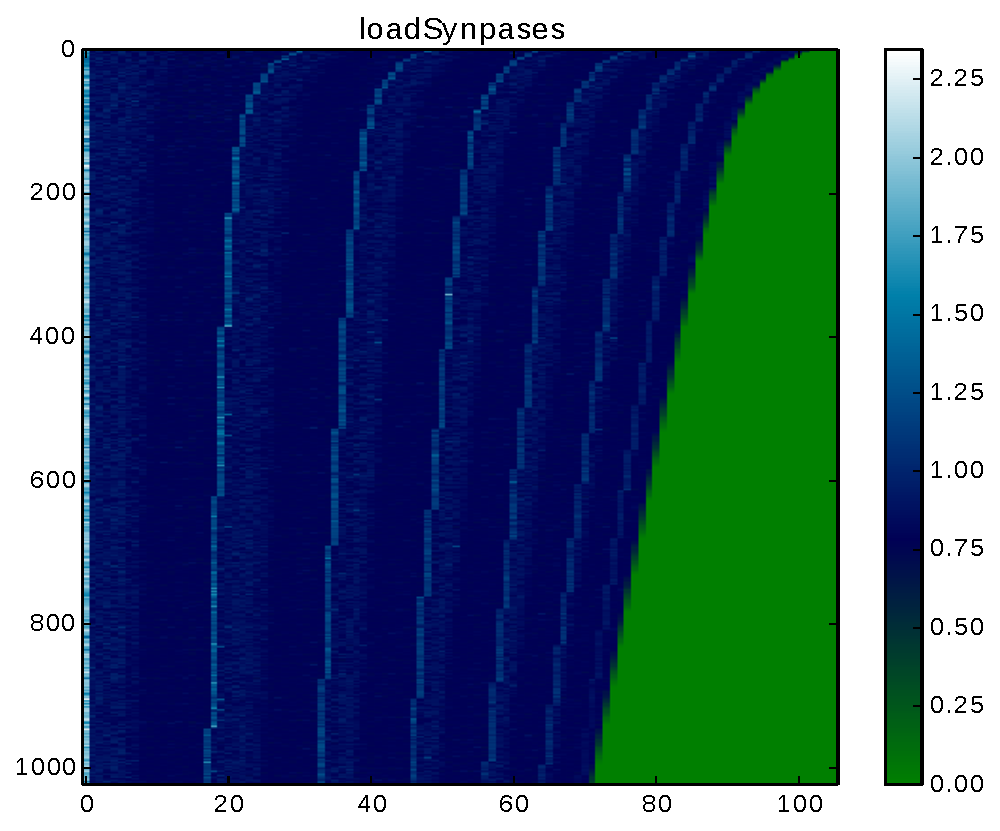
\includegraphics[width=0.45\textwidth]{pictures/V03_loadSynapses.eps}
%        }
%        \subfigure[Sort connection information data by target node]{%
%           \label{fig:second}
%           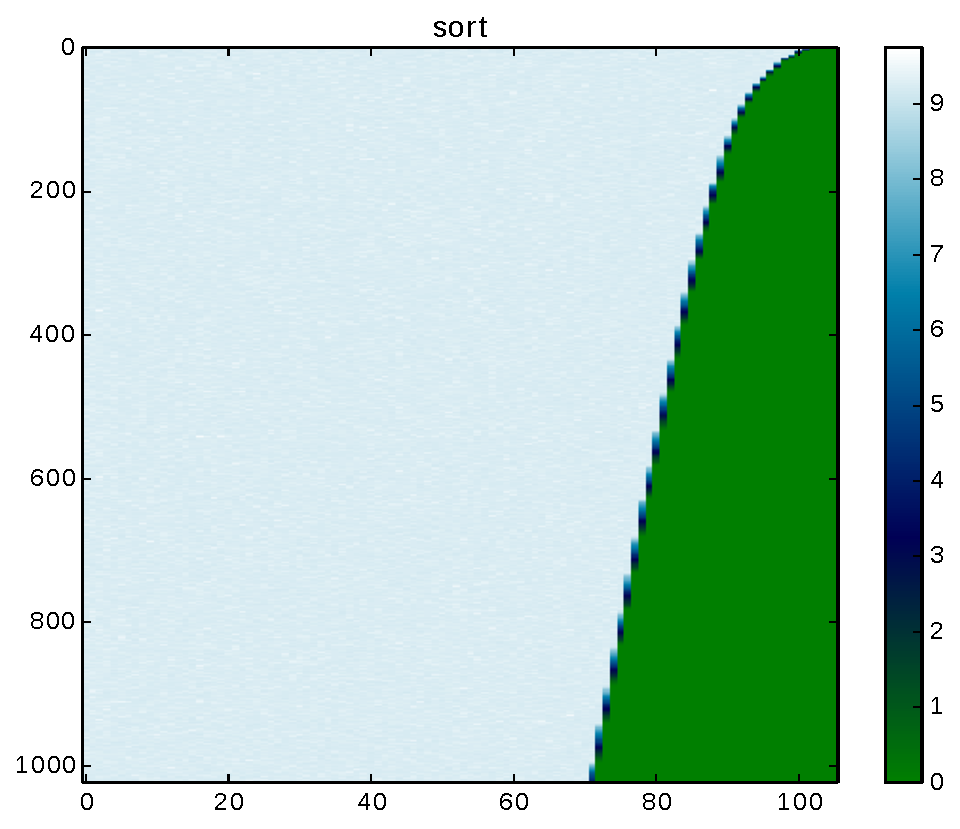
\includegraphics[width=0.45\textwidth]{pictures/V03_sort.eps}
%        }\\ %  ------- End of the first row ----------------------%
%        \subfigure[Send data to all target nodes using AlltoAllv]{%
%            \label{fig:third}
%            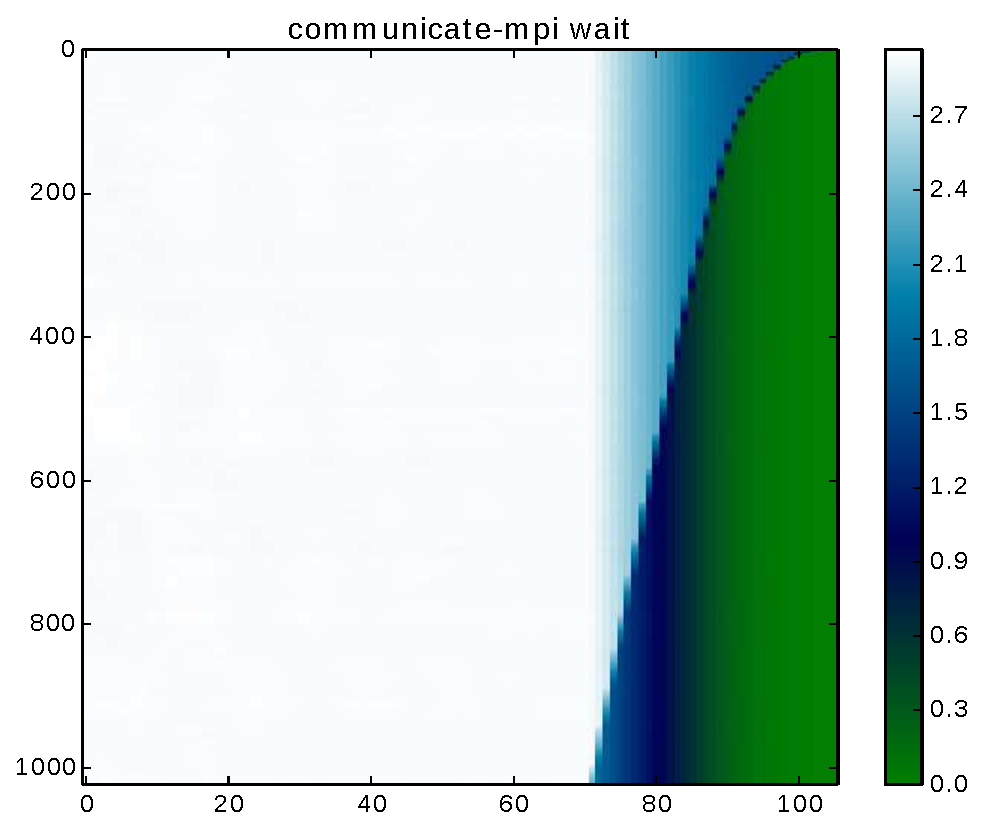
\includegraphics[width=0.45\textwidth]{pictures/V03_communicate.eps}
%        }
%        \subfigure[Connect function which calculated delay and calls NEST connect]{%
%            \label{fig:fourth}
%            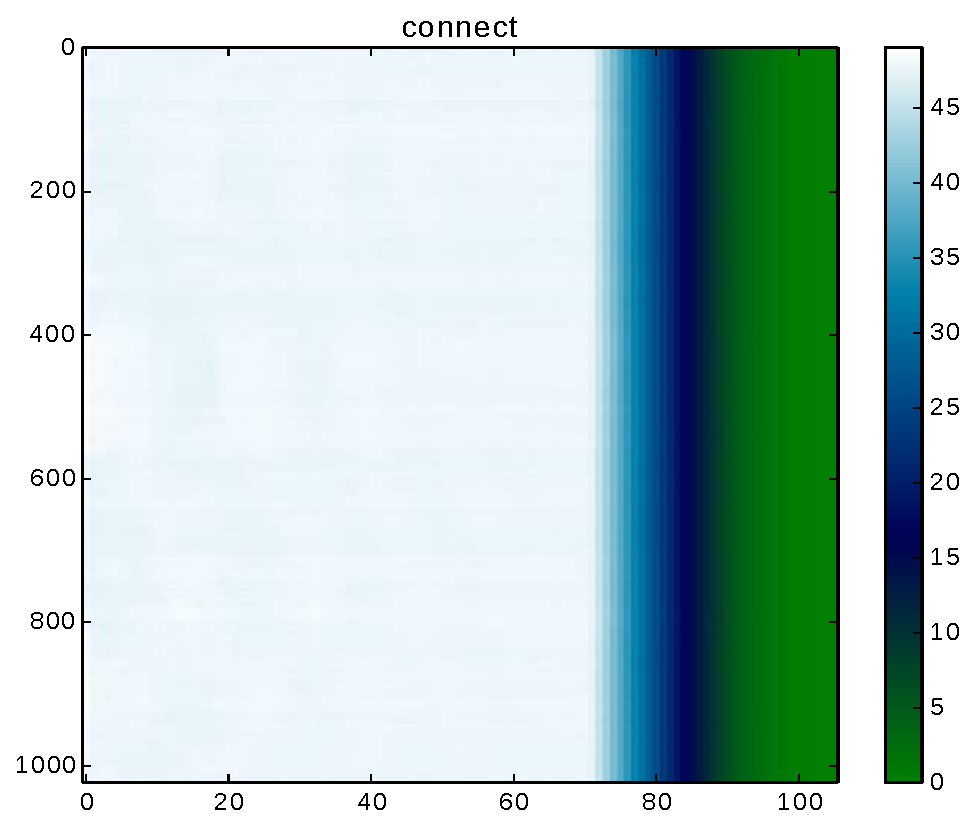
\includegraphics[width=0.45\textwidth]{pictures/V03_connect.eps}
%        }
%    \end{center}
%    \caption{%
%        The the plots show the the execution time for node per iteration.
%        The y-axes corresponds to the node id and the x-axes corresponds to the iteration number.
%        The color scale is in seconds.
%        In each iteration loadSynapses loads max $1e6$ synapses from hdf5 file.
%     }%
%   \label{fig:implV03}
%\end{figure}
One can see that \emph{Read} and \emph{Connect} are the critical parts.
For the interpretations of the plots one has to take into account that different parts of the algorithm
(\emph{Read} and \emph{Alltoall}) contain mpi collective operations and contain therefor mpi waits.
Thus the wall-clock timings do not satisfy the pure step duration but also the imbalance from previous steps.
To analyse the impact, an experiment is performed which extends the implementation with \emph{MPI\_Barriers}
between the algorithm steps.
\newpage
\subsection{Read step}
The efficiency of the \emph{Read} step is bounded by the io bandwidth of the system.
Blue Brain IV has a theoretical bandwidth of $50$ GB/s per rack.

The amount of data read in \emph{Read} step depends on the number of synapse parameters $N_{params}$,
the number of read synapses per iteration $N_{blocksize}$ and the number of processes $N_{processes}$.
This results in a measured bandwidth of:
\begin{equation}
b = sizeof(float) * N_{params} * \frac{N_{blocksize} * N_{processes}}{\Delta T}
\end{equation}
\subsection{Connect step}

Thread parallelization of the connect step allows to store the synapses efficiently in the NEST data structure.
The pure connect functionality of NEST is thread-safe. But creating and destroying SLI data objects is not and can result
in data-races. To overcome this limitation the creation and destroying of the objects is serialized.
Before iterating over all synapses one SLI object is created and destroyed afterwards for each thread.
A single connect function call of the NEST api expects the synapse parameters stored in a SLI object.
In each iteration the current parameters are assigned to the values inside the already created SLI object.
This SLI object is passed to the function call.
Thus a small overhead for the creation and destroying of the object are perceived.
\begin{figure}[ht!]
\centering
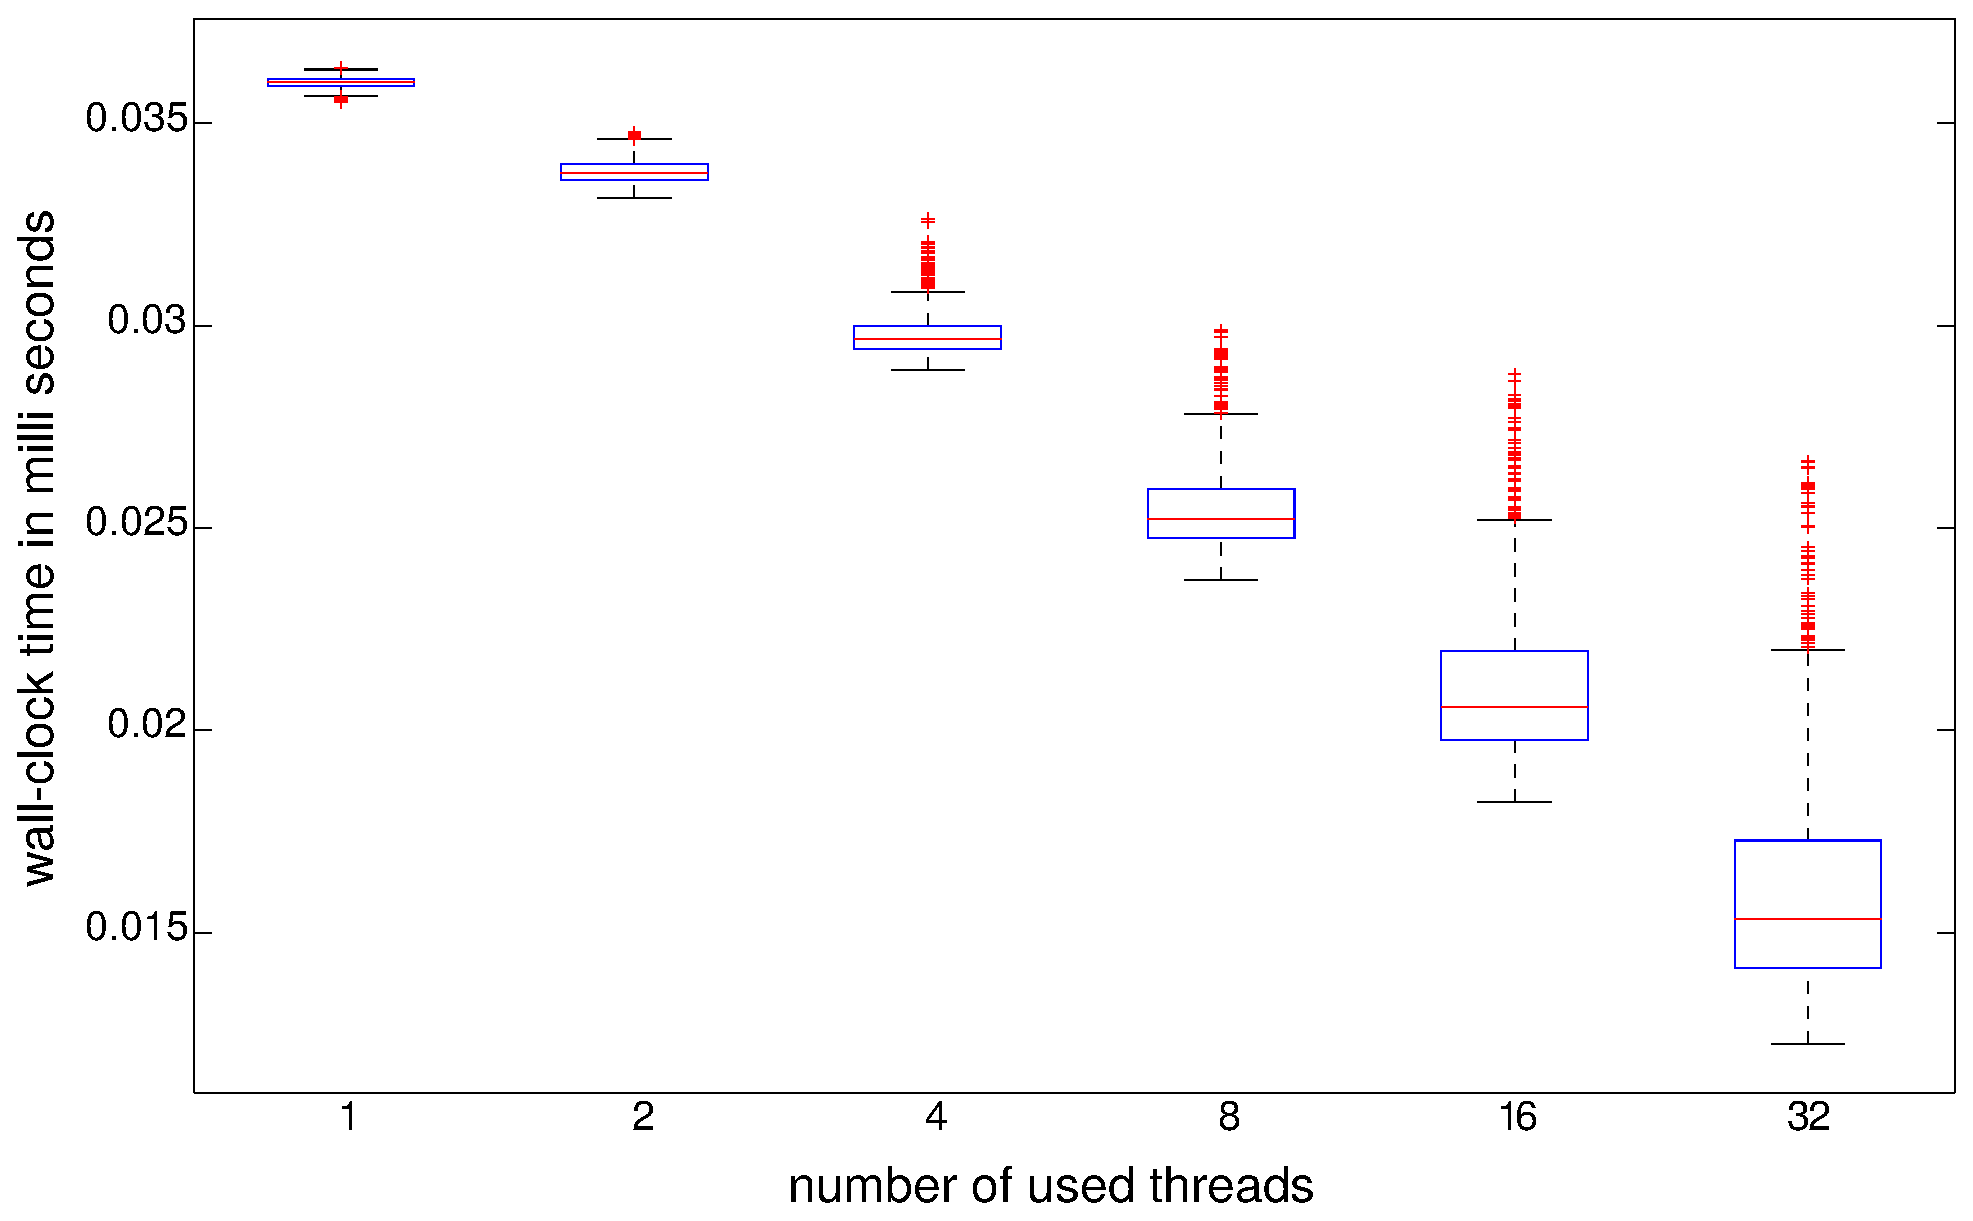
\includegraphics[scale=0.3]{pictures/boxplot_new_con_dt_1_300_edit.eps}
\caption{Comparison of mean of single connect duration across one iteration on one node.}
\label{boxplotnewcon}
\end{figure}
Because each thread iterates over all synapses, but only stores the connection if the post-synaptic neuron is located on
the thread, the connection calls per thread varies.
As for nodes the neurons are distributed in the modules fashion on the threads for one node.
The distribution properties are the same. Thus there is a larger variation on a larger number of threads.
Figure \ref{boxplotnewcon} shows wall-clock time measurements for the connect step. The measurements are
extracted from the execution of the threehundredths circuit. It is executed on 128 nodes with varying number of
threads. The circuit plus fixed number of nodes specify the distribution of neurons per node.

A larger number of threads leads to smaller wall-clock timings, but the chance of imbalance increases.
The variations of the timings correlates with the distribution of synapses per node (figure \ref{fullcircuitdist}).
To look into detail, figure \ref{detailnewcon:second} shows the measured wall-clock time for each node
plotted over the maximum number of new connections per thread. It shows a strong correlation between the variable and
the duration. Thus the increasing variations of timings can be explained by the variations of synapses per thread.
The figure indicates two different timings per connection. There is an offset of regression between the pink
(left point cloud)
and the red (right point cloud) dots. Pink an red dots represent all measurements with less than 40,000 and more than new synapses per
node respectively. Figure \ref{detailnewcon:first} shows the density of number of new synapses per node.
Less synapses results in a smaller vector size. There seems to be a loss of efficiency, which properly result from
the use of different cache levels. 

\begin{figure}[ht!]
     \begin{center}
        \subfigure[Histogram showing measured densities of number of new synapses per iteration step for one process.]{%
            \label{detailnewcon:first}
            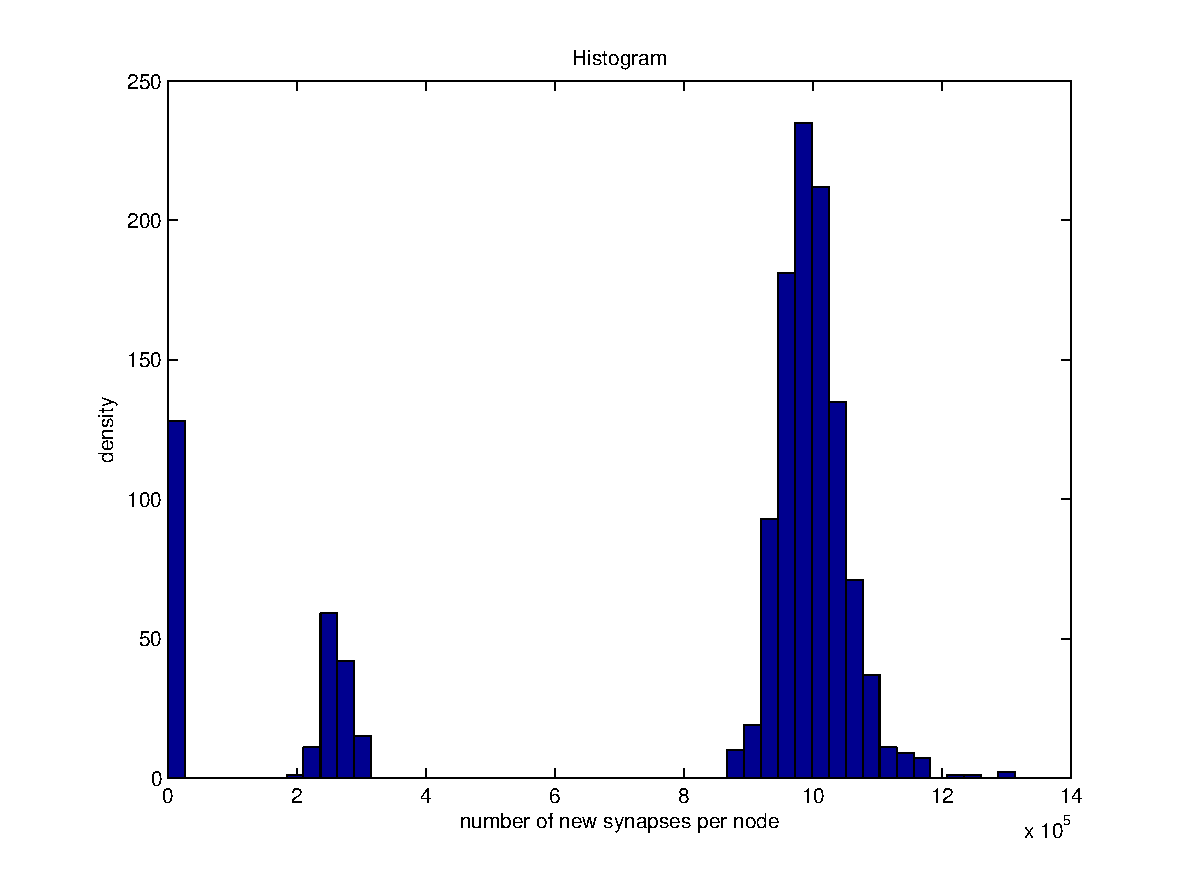
\includegraphics[scale=0.41]{pictures/histogram_new_const_1_300.eps}
        }
        \subfigure[Plotted wall-clock timings of \emph{connect} step over the number of new synapses for one thread
        			(Thread is part of process from Figure \ref{detailnewcon:first}. The new synapses are part of the new synapses from the process).
        			Pinks and red dotes relate to iterations, where the number of new synapses is smaller and bigger than $4*10^5$,
        			respectively (The values relate to the hills from Figure \ref{detailnewcon:first}). 
        			]{%
           \label{detailnewcon:second}
           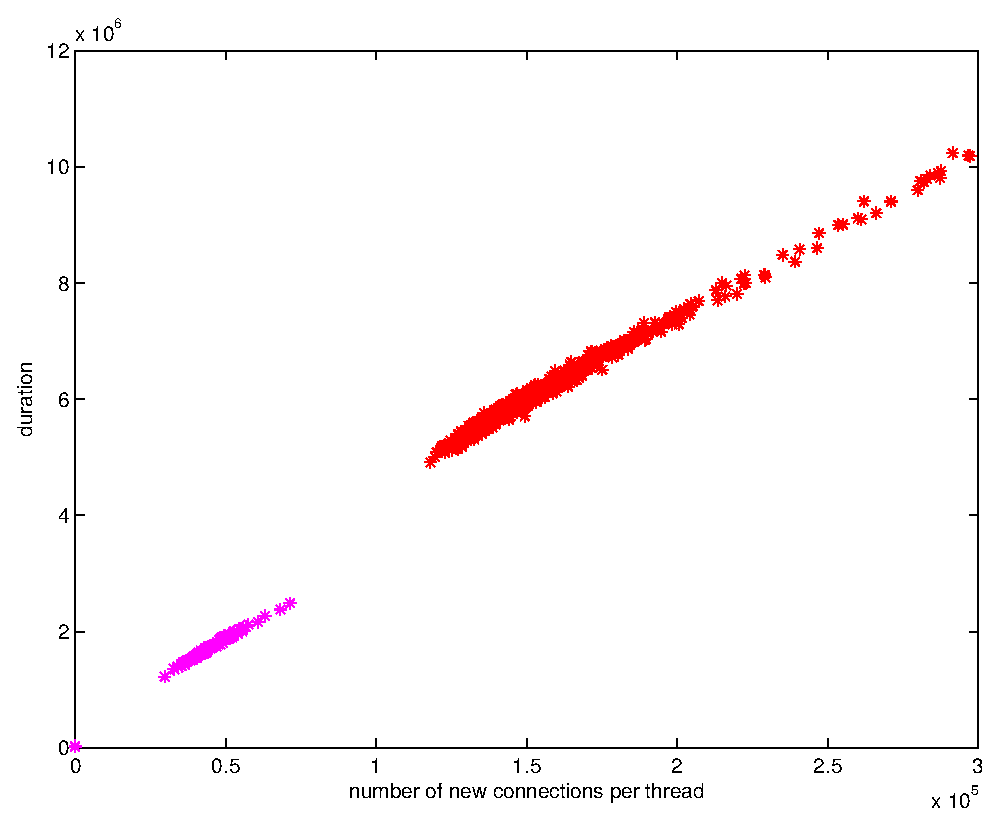
\includegraphics[scale=0.41]{pictures/t8_duration_per_con_1_300.eps}
		}
    \end{center}
    \caption{%
        The measurements are taken the same simulation run with the 1per300 circuit. It is run on the Blue Brain IV.
     }%
   \label{detailnewcon}
\end{figure}

%\begin{figure}[!h] \centering
%\begin{tikzpicture}
%	\begin{axis}[title=AMBM CONNECT MODULE,
%		legend style={at={(0.5,-0.20)},
%		anchor=north,legend columns=-1},
%		xlabel=number of racks,
%		ylabel=Parallel efficiency (\% of linear scaling),
%		width=8.5cm
%		]
%
%	\addplot[color=blue,mark=*] coordinates {
%		(1,100)
%		(2,110)
%		(4,30)
%	};
%	\addplot[color=red,mark=*] coordinates {
%		(1,100)
%		(2,114)
%		(4,117)
%	};
%	\addplot[color=green,mark=*] coordinates {
%		(1,100)
%		(2,84)
%		(4,54)
%	};
%	\addplot[color=yellow,mark=*] coordinates {
%		(1,100)
%		(2,91)
%		(4,110)
%	};
%	\legend{io,sort,mpi,connect}
%	\end{axis}%
%\end{tikzpicture}%
%\begin{tikzpicture}
%	\begin{axis}[title=AMBM CONNECT MODULE,
%		legend style={at={(0.5,-0.20)},
%		anchor=north,legend columns=-1},
%		xlabel=number of racks,
%		ylabel=wall clock in seconds,
%		width=8.5cm
%		]
%
%	\addplot[color=blue,mark=*] coordinates {
%		(1,73)
%		(2,33)
%		(4,60)
%	};
%	\addplot[color=red,mark=*] coordinates {
%		(1,85)
%		(2,37)
%		(4,12)
%	};
%	\addplot[color=green,mark=*] coordinates {
%		(1,278)
%		(2,163)
%		(4,132)
%	};
%	\addplot[color=yellow,mark=*] coordinates {
%		(1,171)
%		(2,93)
%		(4,38)
%	};
%	\legend{io,sort,mpi,connect}
%	\end{axis}%
%\end{tikzpicture}%
%\end{figure}
%\begin{figure}[!h] \centering
%\begin{tikzpicture}
%	\begin{axis}[title=AMBM NEST RUN,legend style={at={(0.5,-0.20)}, anchor=north,legend columns=-1},
%		xlabel=number of racks,ylabel=Parallel efficiency (\% of linear scaling),width=8.5cm]
%
%	\addplot[color=blue,mark=*] coordinates {
%		(1,100)
%		(2,93)
%		(4,72)
%	};
%	\addplot[color=red,mark=*] coordinates {
%		(1,100)
%		(2,94)
%	};
%	\addplot[color=red,mark=o] coordinates {
%		(1,100)
%		(2,94)
%		(4,101)
%	};
%	\legend{mod,slisim, slisim estimated}
%	\end{axis}%
%\end{tikzpicture}%
%\begin{tikzpicture}
%	\begin{axis}[title=AMBM NEST RUN,legend style={at={(0.5,-0.20)}, anchor=north,legend columns=-1},
%		xlabel=number of racks,ylabel=wall clock in seconds,width=8.5cm]
%
%	\addplot[color=blue,mark=*] coordinates {
%		(1,640)
%		(2,344)
%		(4,220)
%	};
%	\addplot[color=red,mark=*] coordinates {
%		(1,1208)
%		(2,637)
%	};
%	\addplot[color=red,mark=o] coordinates {
%		(1,1208)
%		(2,637)
%		(4,299)
%	};
%	\legend{mod,slisim, slisim estimated}
%	\end{axis}%
%\end{tikzpicture}%
%\end{figure}

\section{Measured memory consumption}

\subsection{Long range connection generation}



\subsection{Short range connection generation}
\subsection{Load circuit}

\newpage
\section{Usability for Scientists}

\subsection{Manipulation of circuit}

\begin{itemize}
      \item control circuit generation / possibilities
      \item  manipulate circuit
\end{itemize}

\subsection{Import neurons}
\emph{H5NeuronCsX\_s\_s\_a\_s} expects 4 input parameters:
\begin{itemize}
      \item Name of the a subnet dataset (String).
The subset has to contain for each neuron an integer value.
The neurons are grouped together by this subnet value.

      \item A list of all datasets which values are interpreted as list of parameters.
      
      \item Name of the used neuron model
      
      \item path to the HDF5 file 
\end{itemize}
The function returns the neuron id of the first neuron it created.

\begin{lstlisting}[label=sliNeurons,caption=Calling the neuron import module via H5NeuronCsX\_s\_s\_a\_s SLI command ]
/neuronmodel /aeif_cond_exp def
/subnet (subnet) def
/neuronparams [(C_m) (Delta_T) (E_L) (V_reset) (V_th) (a) (b)] def
/filepath (circuit/ptneu_brain.h5) def
subnet neuronparams neuronmodel filepath H5NeuronCsX_s_s_a_s /offset Set
\end{lstlisting}



\begin{itemize}
      \item Sli command with parameters
      \item How can it be used
\end{itemize}

\subsection{Import synapses}
\emph{H5SynapseTll\_i\_s\_a\_s} expects 4 input parameters:
\begin{itemize}
      \item Offset of the neuron ids. Mostly it is equal to first neuron id returned by \emph{H5NeuronCsX\_s\_s\_a\_s}

      \item A list of all columns which values are interpreted as parameters.
      
      \item Name of the used synapse model
      
      \item path to the HDF5 file 
\end{itemize}
The function returns the neuron id of the first neuron it created.

\begin{lstlisting}[label=sliSynapses,caption=Example importing synapses]
/synmodel /tsodyks2_synapse def
/synparams [(delay) (weight) (U0) (TauRec) (TauFac)] def
/filepath (circuit/syn.h5) def
offset synparams synmodel filepath H5SynapseTll_i_s_a_s
\end{lstlisting}
\begin{itemize}
      \item How can it be used
\end{itemize}

\subsection{NEST simulation options}

Only one use-case (\ref{s}) of the mouse brain model is used in this thesis for performance evaluations.
Never the less more use-cases are realizable with the given implementations.
In general the neuron load module can be used equivalent to the neuron create function
and the synapses load module can be used equivalent to the neuron connect function.
Further a given circuit can be loaded and adapted (use offset or scaling factor for parameters).
Load neurons can be divided into subsets. The SLI functionality allow to access neuron sets
from the subnets. Thus the grouping performed with the subnet dataset is available for all SLI functions.
Stimulus generator and \emph{Spikedetector} or \emph{Multimeter} can be used to stimulate
and observe specific neurons respectively.
Furthermore SLI connect functions can be used to strengthening or weakening the connections between to
parts of the circuit.

\begin{itemize}
	  \item Test different stimuli
	  \item how to get results
\end{itemize}

\subsection{Analysis}
\begin{itemize}
	  \item Visualize spiking activity with Brion/Paraview
      \item Visualize spiking activity with ViSNEST
\end{itemize}


%%%%%%%%%%%%%%%%%%%%%%%%%%%%%%%%%%%%%%%%%%%%%%%%%%%%%
% Der Anhang (andere Sektionsnummerierung)
%%%%%%%%%%%%%%%%%%%%%%%%%%%%%%%%%%%%%%%%%%%%%%%%%%%%%
\appendix
% Hier werden die Anhänge eingebunden
% TODO : weitere Kapitel in my_appendices.tex eintragen
\input{my_appendices.tex}

\bibliography{gesammelte_werke} %Literaturverzeichnis
\bibliographystyle{abbrv}       %Stil des Literaturverzeichnisses (en)
%\bibliographystyle{abbrvdin}       %Stil des Literaturverzeichnisses (de)

% evtl. Abkuerzungsverzeichnis (z.B. Paket nomenclature)

\printindex                     % Wenn ein Index erstellt werden soll, muss
                                %  diese Zeile aktiviert werden
                                %  Zusaetzlich oben das Paket einbinden und \makeindex

\end{document}



